\documentclass{article}
\usepackage{graphicx} % Required for inserting images
\usepackage[top=1.2in, bottom=1.2in, left=3cm, right=3cm, a4paper]{geometry}
\usepackage{subcaption}
\usepackage{ragged2e}
\usepackage[hidelinks]{hyperref}
\hypersetup{
	colorlinks=true,
	linkcolor=blue,
	filecolor=blue,      
	urlcolor=blue,
	citecolor=black,
}
\usepackage{amsmath}
\usepackage{listings}
\usepackage{natbib}
\begin{document}

\thispagestyle{empty}
\begin{center}
    	\begin{figure} [t]
		
\includegraphics[width=0.2\linewidth]{../fig/logo_UGA.png}
		\hspace{8.0cm}
		
\includegraphics[width=0.2\linewidth]{../fig/logo_IGE.png}
		\vspace{2.0cm}
	    \end{figure}

        \begin{Large}
        \textbf{Numerical experiments in glacial inceptions in Northern Europe} 
        \end{Large}
        
        \vspace{0.8cm}
        \textbf{ESPELETA BOLIVAR, Ruben Dario}\\
        \vspace{3.0cm}
        \textbf{Research project}\\
	    Presented in partial fulfillment of the requirements for the degree of\\
	    \textbf{Master applied mechanics}\\
        \vspace{3.0cm}

        Université Grenoble Alpes\\
        \textbf{\today}
        \vspace{4.0cm}
\end{center}
\flushleft{
    Project advisor(s):\\
    Ph.D. Cruz García Molina
}
\clearpage

\begin{center}
	\textbf{\Large{Abstract}}
\end{center}

\vspace{0.5cm}

\justifying

The present project aims to develop a numerical experiment to understand the impact of important parameters in the glacier dynamics, such as the grounding line. Using the finite element method Elmer/Ice, simulations on idealized topographies are proposed, which are set up in the context of the CalvingMIP inter-comparison project, that aims to develop different models to simulate and to improve calving laws in ice sheet models. Using these idealized topographies, the numerical experiments are performed using resolutions varying from 10km until 1km, starting from an initial state where there is no ice, until the formation of the glacier. The objective of the study is to evaluate the impact of the resolution on the prediction of the grounding line position after the system has reached the steady state. The analysis of the results are contrasted with the theory and show the convergence of the behaviour of the grounding line position for higher resolutions, where the differences start to be lower.

\vspace{3cm}

\clearpage
\tableofcontents

\pagebreak

\section{Introduction}
\justifying
Glaciers can be defined as a mass of ice that accumulates from snow and flows slowly downwards. The ice sheets are very large mass of this ice of continental scale that flows outwards \cite[]{anesio2012glaciers}. Some representative examples are Antarctic and Greenland ice sheets. Ice sheets are important components of global climate systems \cite[]{zhang2017comparison}. The perturbation of these climate systems has several impacts for example, changes in global sea level, as ice sheets grow or decay in response to climate forcing and internally controlled dynamics. The rate of present-day sea-level rise is dominated by ocean steric changes (namely, the ocean expansion due to ocean water molecules expansion) and eustatic changes (namely, expansion of the ocean due to the addition of water) due to shrinking mountain glaciers, and the eustatic contribution from the large ice sheets (Greenland and Antarctic) has increased in recent decades and it is expected to continue increasing in coming decades and centuries \cite[]{clark2015recent}. For example, \cite{morlighem2017bedmachine} and \cite{haywood2011pliocene} mentioned that if all the ice were to melt completely, the sea level would rise by an estimated of 65m. Also the Unites Nations states that around 40\% of the world's population lives in coastal regions, within 100km of the coastline \cite[]{barbier2015climate, montgomery2007united}. The land area that is less than 10m above sea level is just 2\% of the world's total land area, yet it is home to 10\% of the world's population and 13\% of the world's urban population \cite[]{nevermann2023land}. This indicates the amount of population that could be affected by a sea level rise of this magnitude. 

However, even if an estimate of the amount of ice present in the glaciers is known, such as the Antarctic and Greenland, for example, the changing dynamics of these are not well known, mainly due to the changing parameters and environmental phenomena that play an important role in the dynamics of the glaciers.

In order to understand these impacts on the dynamics and melting of ice sheets and glaciers, numerical models are developed. These models are a simplification of reality, and they represent physical real-world processes by a series of equations, which can be solved to understand how the system will respond under different scenarios. The figure \ref{Modelling_process} shows a scheme where the modelling process is described. The mathematical description of a physical process or phenomena can be discretized to be then solved numerically, using a numerical method. However, these mathematical models are usually complicated to discretized or solved numerically, due to the complexity of the differential equations. For this reason, different approximations can be implemented to represent ice flow dynamics that allows to make certain simplifications to these equations. 

\begin{figure}[!h]
	\centering
	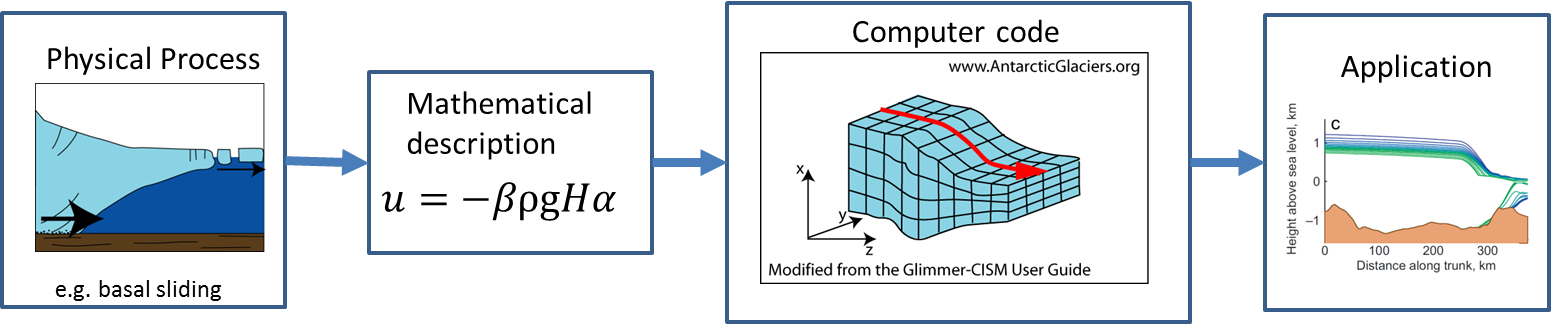
\includegraphics[width=0.7\linewidth]{../fig/Numerical_modelling_scheme.png}
	\caption{Process of modelling starting with a physical process which can be described mathematically and turned into a computer code where discretized equations are solved numerically.}
	\label{Modelling_process}
\end{figure}

The different approximations that can be done to the mathematical models that described the glacier dynamics are presented in this document, where the equations of motion will be presented in the next section. Also, the different numerical methods that can be used to solved the approximations of these mathematical methods will be also introduced.  

\begin{figure}[!h]
	\centering
	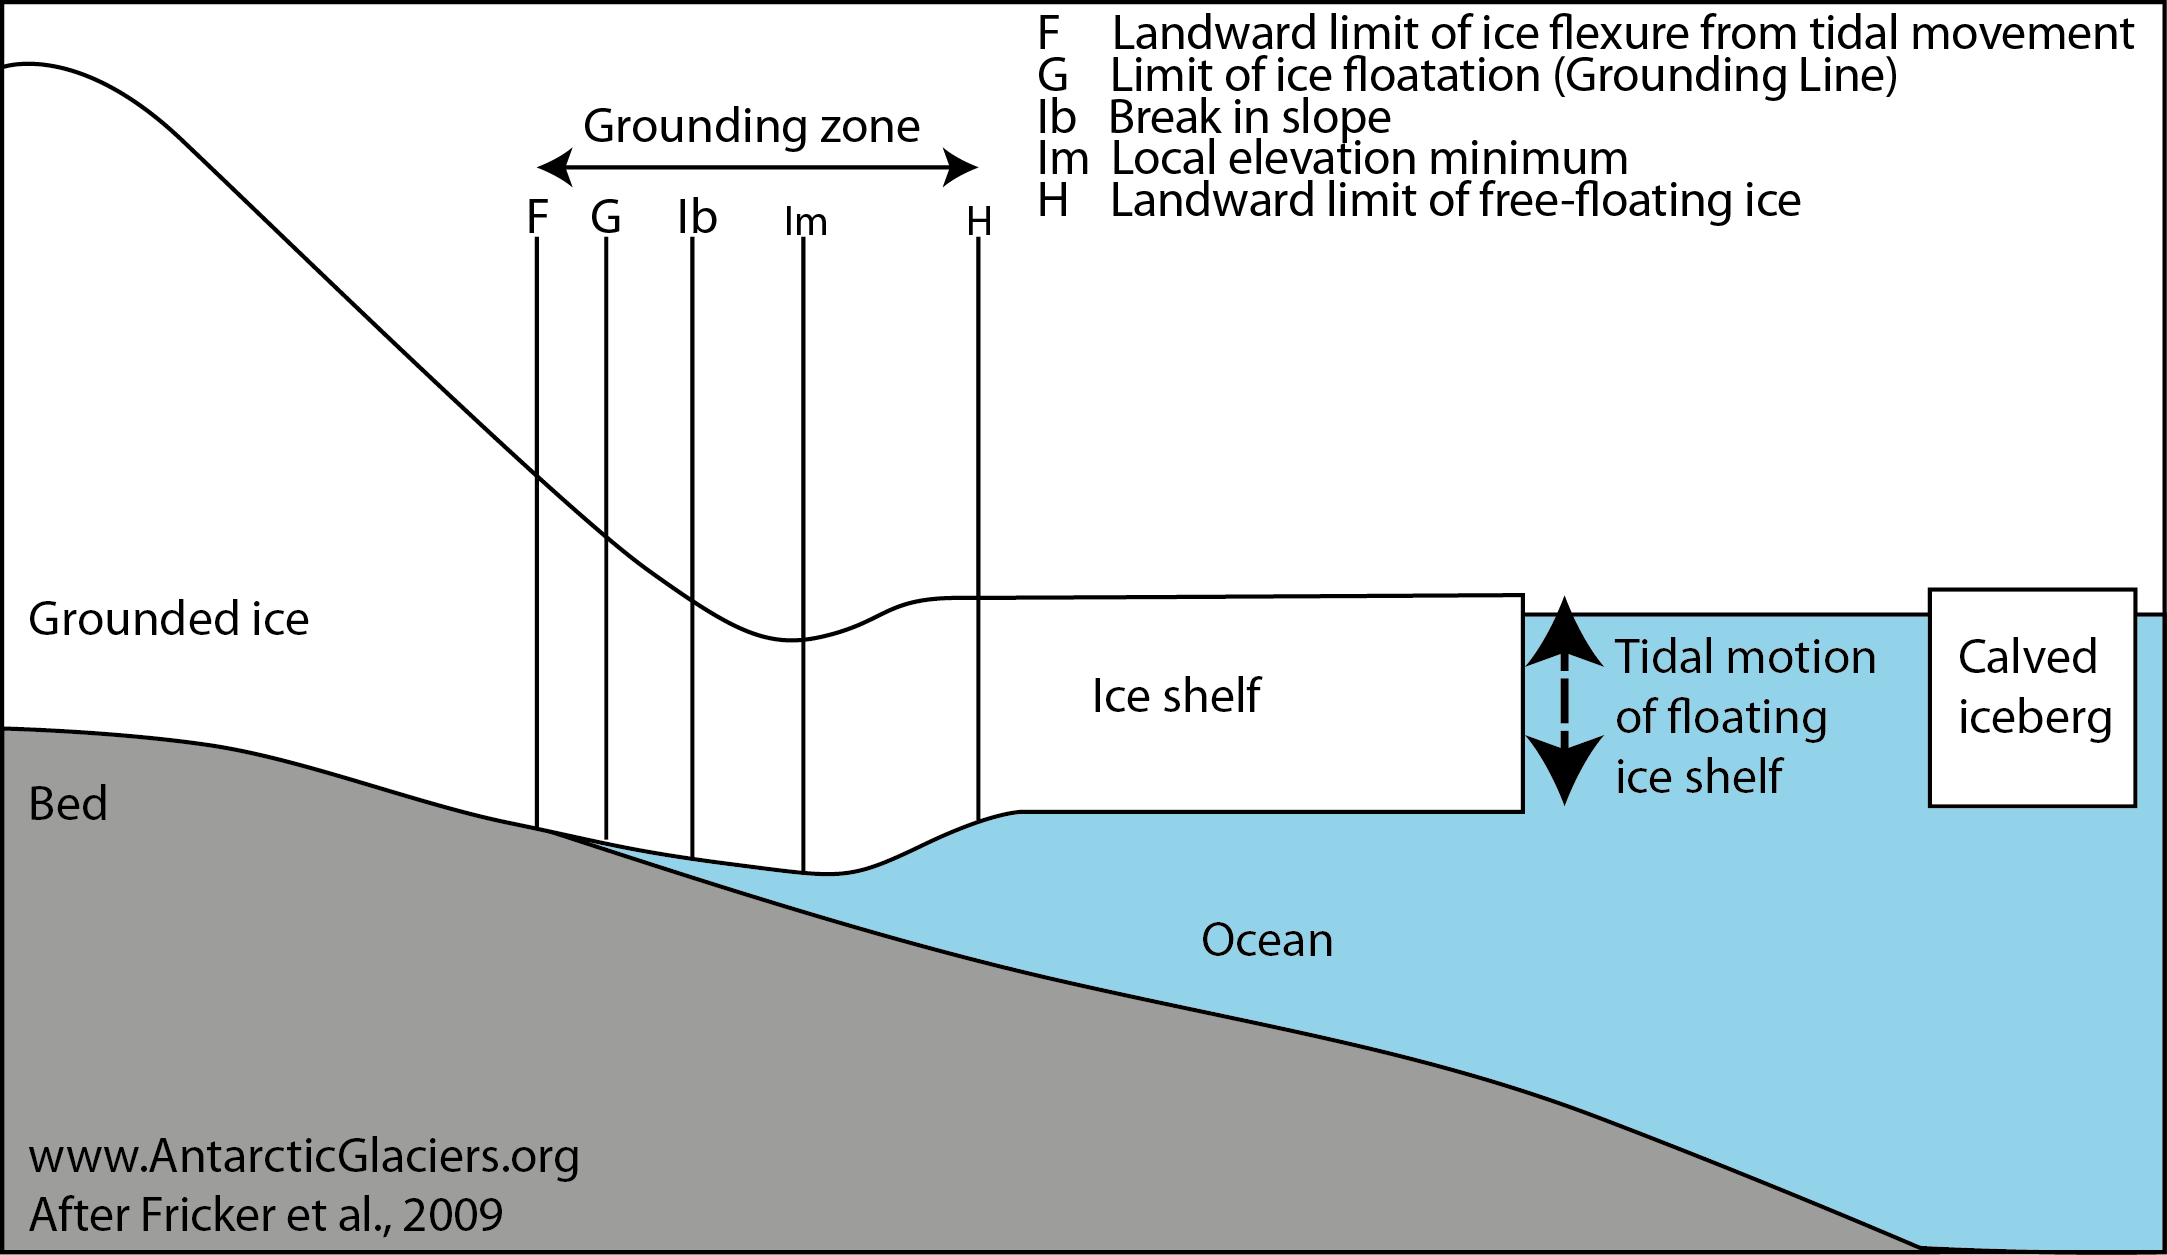
\includegraphics[width=0.7\linewidth]{../fig/groundingzone.png}
	\caption{Schematic of a tributary glacier where we can observe the different parts denoting the grounding zone \cite[]{fricker2009mapping}.}
	\label{groundingzone}
\end{figure}

Glaciers can be classified in different types. Glaciers that end in the ocean are called tidewater glaciers. The ones that flow into an ice shelf are called tributary glaciers as the one shown in figure \ref{groundingzone}. The zone that divides the part of the glacier that is in contact with the solid bedrock and the ice shelf floating on water driven by buoyancy, is called the grounding line \cite[]{cheng2019full}. The location of the grounding line is important because the mass loss from glaciers is strongly linked to changes in the ice shelves and their grounding lines \cite[]{brunt2010mapping,pritchard2012antarctic}. Its long-term horizontal position is very susceptible to temporal and spatial changes in ice thickness and sea level, as well as bedrock and ice surface slopes. Ice thinning and rising sea levels can cause grounding lines to retreat while thickening or declining sea levels can cause an advance \cite[]{friedl2020remote}. It is important to know the grounding line position to be able to quantify the ice discharge into the sea and as an indicator, if the ice sheet is advancing or retreating \cite[]{konrad2018net}.

Grounding lines are actually more of a zone or region where ice transitions from a grounded ice sheet to a freely floating ice shelf, typically over several kilometres. A schema of the grounding zone is shown in figure \ref{groundingzone}. In this figure, the grounding zone is the region between point F, where there is no tidal movement, and point H, which is the seaward limit of ice flexure, where the ice is free-floating. The floating ice shelf changes in elevation in response to tides, atmospheric air, pressure, and oceanic processes. Grounding occurs when the ice shelf comes into contact with the bedrock below \cite[]{fricker2009mapping}. The transition from grounded ice sheets to floating ice shelves plays an important role in controlling marine ice sheet dynamics, as it determines the rate at which ice flows out of the grounded part of the ice sheet \cite[]{schoof2007ice}. This is because ice flux through the grounding line increases sharply with ice thickness at the grounding line. This means that grounding lines are unstable on reverse-bed slopes, such as those under Pine island glaciers, because recession into deeper water increases ice flux and further encourages more glacier recession \cite[]{schoof2007marine}.

In section \ref{glacier_dynamics} the dynamics of the glacier will be introduced and the governing equations are presented. The stability conditions for the position of the grounding line is presented in section \ref{grounding_line_stability}. A literature review on the grounding line position studies is presented in section \ref{grounding_line_stability} too, where the impact of parameters such as the mesh resolution on the prediction of the grounding line position is discussed and presented as a research opportunity for the present study that aims to understand and to obtain reliable models able to predict this grounding line dynamics, by implementing experiments on glacier dynamics through idealized topographies. An introduction about the different numerical methods that are used in glaciology to solve the mathematical models that govern the glacier dynamics is presented in section \ref{Numerical_methods} and in section \ref{Numerical_model} the Elmer/Ice method is described. The idealized topographies that are proposed for the experiments driven in this project are presented in section \ref{Systems}. These idealized topographies are proposed in the context of the CalvingMIP inter-comparison project, which has been developed with the purpose of proposing different models to simulate and to improve calving laws in ice sheet models, and is detailed in section \ref{Systems}. The main results of the experiments driven in this project are presented in section \ref{Results}, where the steady state results of the simulations are presented and the comparison of the grounding line position for each resolution mesh is shown, allowing to show the convergence of the steady state grounding line position as the mesh resolution increases and to show the impact of the bedrock topography on the accuracy of the model to predict the grounding line position. 

\section{Glacier dynamics}
\label{glacier_dynamics}
\subsection{Mass and movement balance equations}
An ice sheet is a continuous sheet of land ice that covers a very large area of several thousand to millions of square meters. It is formed by an accumulation of snow which will densify under its own weight until it becomes ice. This ice will then flow downhill under its weight, and can eventually reach the sea. If it does, and the ice propagates above the sea, this part of the ice sheet is called an ice shelf \cite[]{hutter1982mathematical}. Figure \ref{groundingzone} shows a diagram of an ice sheet showing different parts of it, such as the ice shelf, and the grounded ice. The grounding zone can also be identified. 

Figure \ref{control_volume} shows an elementary control volume of ice in a glacier, of size $dx.dy.dz$. The velocities into the volume in the $x$, $y$ and $z$ directions are $u$, $v$, and $w$, respectively. The velocity out in the $x$-direction is:

\begin{equation}
	U = u+\frac{\delta u}{\delta x}dx;
\end{equation}

\begin{figure}[!h]
	\centering
	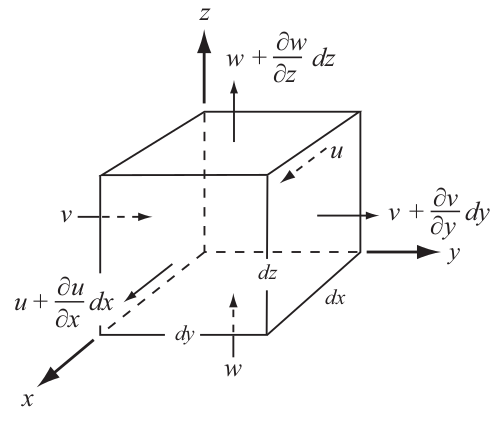
\includegraphics[width=0.5\linewidth]{../fig/Control_volume.png}
	\caption{Derivation of the condition of incompressibility. Adapted from \cite{hooke2019principles}.}
	\label{control_volume}
\end{figure}

Here, $\frac{\delta u}{\delta x}$ is the velocity gradient through the volume, which, when multiplied by the length of the volume, $dx$, gives the change in velocity through the volume in the $x$-direction. The mass fluxes into and out of the volume in the $x$-direction are:
\begin{equation}
	({\rho u + \frac{\delta \rho u}{\delta x}dx})dy dz;
\end{equation}

Here, $\rho$ is the density of the ice. Similar relations may be written for the mass fluxes into and out of the volume control in the $y$ and $z$-directions. Summing these fluxes we find that the change in mass with time, $\frac{\delta m}{\delta t}$ in the control volume is:

\begin{equation}
	\frac{\delta m}{\delta t}=\rho u dydz-({\rho u+\frac{\delta \rho u}{\delta x}})dydz-({\rho v+\frac{\delta \rho v}{\delta y}})dxdz+\rho vdxdz+\rho wdxdy-({\rho w+\frac{\delta \rho w}{\delta z}})dxdy;
\end{equation}
Simplifying by cancelling terms of opposite sign and dividing by $dxdydz$ yields to:
\begin{equation}
	-\frac{1}{dxdydz}\frac{\delta m}{\delta t}=\frac{\delta \rho u}{\delta x}+\frac{\delta \rho v}{\delta y}+\frac{\delta \rho w}{\delta z};
\end{equation}
Ice is normally considered incompressible, which means that $\rho$ is constant. This is not true near the surface of a glacier, where snow and firn are undergoing compaction, but to a good approximation is valid throughout the bulk of most ice masses \cite[]{hooke2019principles}. In this case, the equation becomes:
\begin{equation}
	-\frac{1}{\rho dxdydz}\frac{\delta m}{\delta t}=\frac{\delta u}{\delta x}+\frac{\delta v}{\delta y}+\frac{\delta w}{\delta z};
\end{equation}

The mass of ice in the control volume can change if the control volume is not full initially. When it is full of incompressible ice, however, $\frac{\delta m}{\delta t}=0$, and the equation becomes:
\begin{equation}
	\frac{\delta u}{\delta x}+\frac{\delta v}{\delta y}+\frac{\delta w}{\delta z}=0;
\end{equation}

This is the condition of incompressibility; it describes the situation in which neither mass nor density are changing in the volume control, and that will allow to make some simplifications to complement the governing equations that will be introduced in the next sections. 
\subsubsection{Stresses}
A stress is a force per unit area, and has the dimensions Nm$^2$ or Pa. Stresses are vector quantities in that they have a magnitude and direction. Stresses that are directed normal to the surface on which they are acting are called normal stresses, while those that are parallel to the surface are shear stresses. A force applied to a surface at an oblique angle results in both shear and normal stresses on the surface.
As shown in figure \ref{Stress2D}, $\sigma_{XZ}$ is the shear stress in the z‑direction on the plane normal to the $x$-axis. Thus, the first subscript in a pair is the orientation of the normal to the plane on which the stress acts, and the second gives the direction of the stress. The figure \ref{Stress_tensor} shows stress vectors on three faces of a cube. Similar stresses occur on the concealed faces, but they are in the opposite directions. The cube is considered to be infinitesimal, representing, say, a point in a glacier. Thus, stresses on any given face can be regarded as uniformly distributed and constant. To completely describe the state of stress at this point, we need nine stress components; thus: $\sigma_{XX}$, $\sigma_{XY}$, $\sigma_{XZ}$, $\sigma_{YX}$, $\sigma_{YY}$, $\sigma_{YZ}$, $\sigma_{ZX}$, $\sigma_{ZY}$, $\sigma_{ZZ}$. This assemblage of stress vectors is called a second-rank tensor. For comparison, a vector, like velocity, is a first-rank tensor; to describe it we need its components along three coordinate axes, so we need three numbers. Similarly, pressure, a scaler, is a zero-rank tensor; it can be described with only one number, the magnitude of the pressure.
\begin{figure}[!h]
	\centering
	\begin{subfigure}{.5\textwidth}
		\centering
		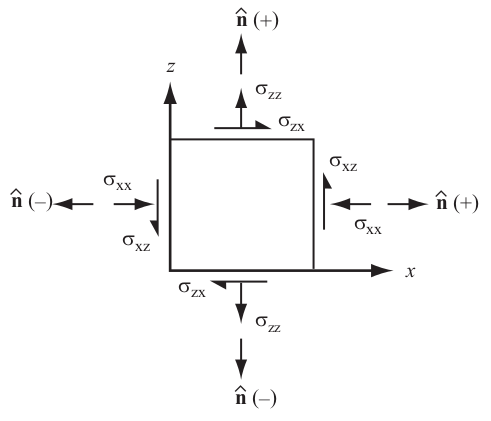
\includegraphics[width=0.99\linewidth]{../fig/Stress_2D.png}
		\caption{Sign convention for stresses in plain strain.}
		\label{Stress2D}
	\end{subfigure}%
	\begin{subfigure}{.5\textwidth}
		\centering
		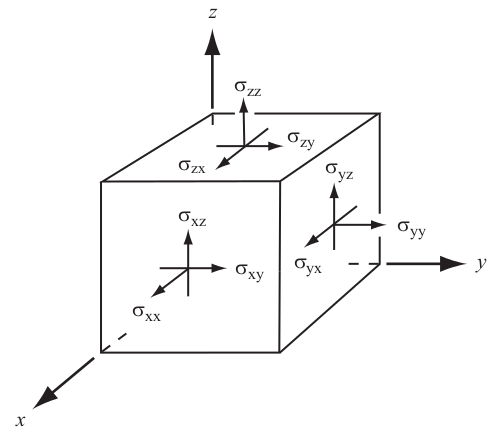
\includegraphics[width=0.99\linewidth]{../fig/Stress_tensor.png}
		\caption{Stresses on a cube.}
		\label{Stress_tensor}
	\end{subfigure}
	\caption{Stress in a elementary control volume of ice. Adapted from \cite{hooke2019principles}.}
	\label{Stress}
\end{figure}

\subsubsection{Strain and strain rate}
In a deformable medium, stresses induce deformation or strain. Strain is defined as the change, $\Delta l$, in length of a line divided by the line's initial length, $\Delta l_0$, thus: $\frac{\Delta l}{l_0}$. The symbol $\epsilon$ is commonly used to denote the strain. The rate at which strain occurs, or the strain rate, $\frac{d\epsilon}{dt}$, is denoted as $\dot{\epsilon}$. As nine separate stress vectors are needed to fully describe the state of stress at a point, so also are nine strains or strain rates needed to describe the state of straining at that point. Thus, these assemblages of strains and strain rates are also second rank tensors, the strain and strain-rate tensors. For the strain rate:

\begin{equation}
	\dot{\epsilon_{XY}}=\frac{1}{2}({\frac{\delta u}{\delta y}+\frac{\delta v}{\delta y}});
\end{equation}

Also, the incompressibility condition can be expressed in terms of the strain rate as:

\begin{equation}
	\dot{\epsilon_{XX}}+\dot{\epsilon_{YY}}+\dot{\epsilon_{ZZ}}=0;
\end{equation}

\subsubsection{Deviatoric stress}

Ice does not deform significantly in response to hydrostatic pressure alone. In other words, in a topographic depression containing ice the hydrostatic (or
cryostatic) pressure increases linearly with depth, $z$, at a rate $\rho gz$, where $g$ is the acceleration due to gravity. As a rule of thumb, the pressure increases at a rate of 0.1 MPa for every 11m of depth. Thus, it becomes quite high at large depths. However, if the surface of the ice in the depression is horizontal, as in a lake, the only deformation that would occur would be a relatively insignificant elastic compression.

On the other hand, if the ice surface were to slope gently (dashed line in
Figure \ref{Deviatoric_stress}), and if points A and B are on a horizontal plane, then the pressure at A would be greater than the pressure at B. This pressure difference would result in a compressive strain between A and B. The strain rate would depend upon the small pressure difference, and not, in any significant way, on the much larger hydrostatic pressure at depth z. In other words, deformation is a result of the non-hydrostatic stresses. It is convenient to define a stress, called the deviatoric stress or stress deviator, which reflects this principle. The deviatoric normal stress in the x-direction is:

\begin{equation}
	\sigma_{XX}'= \sigma_{XX}-P;
\end{equation}

Where P is the mean normal stress:
\begin{equation}
	P=-\frac{1}{3}({\sigma_{XX}+\sigma_{YY}+\sigma_{ZZ}})
\end{equation}

\begin{figure}[!h]
	\centering
	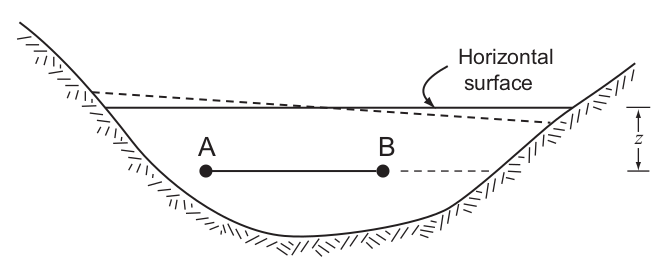
\includegraphics[width=0.7\linewidth]{../fig/Non_hydrostatic_pressure.png}
	\caption{Sketch to illustrate non-hydrostatic pressure. Adapted from \cite{hooke2019principles}.}
	\label{Deviatoric_stress}
\end{figure}

\subsubsection{The flow law}

The most commonly used flow law for ice is Glen’s flow law, named after John
W. Glen upon whose experiments it is based \cite{glen1958flow}. This equation was originally written in the form:
\begin{equation}
	\dot{\epsilon_{e}}=({\frac{\sigma_{e}}{B}})^n;
\end{equation}
where B is a viscosity parameter that increases as the ice becomes stiffer, and n is an empirically determined constant. Most studies have found that n=3¸. An alternative form of the flow law that is commonly used, and that can be used, is:
\begin{equation}
	\dot{\epsilon_{e}}=A\dot{\epsilon_{e}}^n
\end{equation}
A is called the rate factor. B is normally given in Mpa $yr^{\frac{1}{n}}$ while A is in $MPa^{-n} yr ^{-1}$ or $MPa^{-n} s ^{-1}$.

Glaciers move because the surface of the ice is sloped. This generates a stress on the ice, which is proportional to the slope and to the depth below the surface \cite[]{earle2015physical}. As shown in fig \ref{Flow_ice}, the stresses are quite small near the ice surface but much larger at depth, and also greater in areas where the ice surface is relatively steep. Ice will deform, meaning that it will behave in a plastic manner, at stress levels of around 100 kilopascals; therefore, in the upper 50 m to 100 m of the ice (above the dashed red line), flow is not plastic (the ice is rigid), while below that depth, ice is plastic and will flow.

When the lower ice of a glacier flows, it moves the upper ice along with it, so although it might seem from the stress patterns (red numbers and red arrows) shown in figure \ref{Flow_ice} that the lower part moves the most, in fact while the lower part deforms (and flows) and the upper part does not deform at all, the upper part moves the fastest because it is pushed along by the lower ice \cite[]{earle2015physical}.

\begin{figure}[!h]
	\centering
	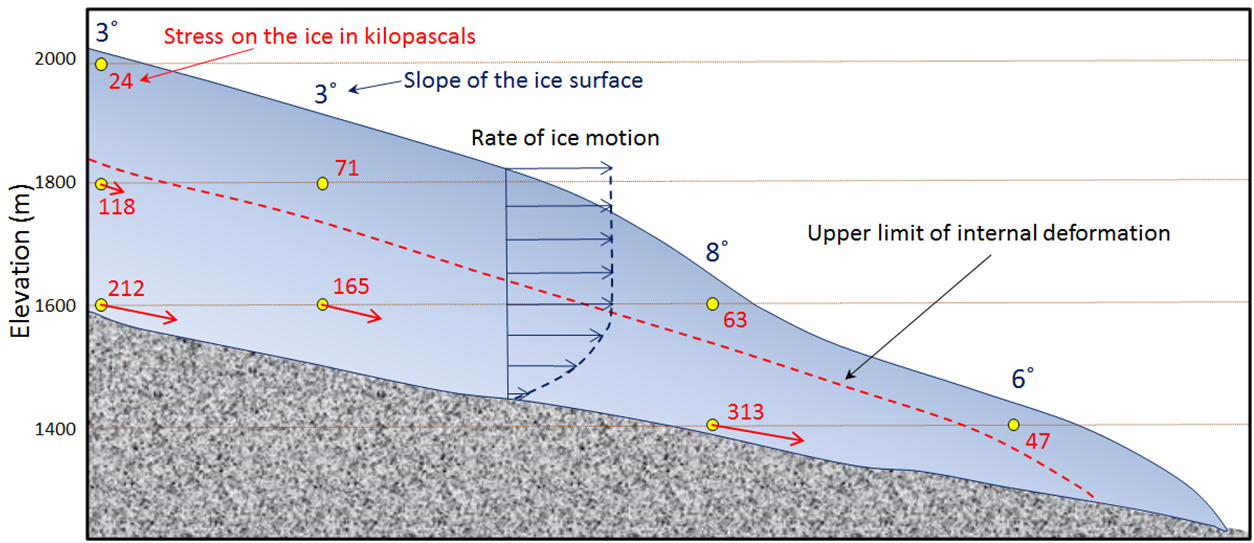
\includegraphics[width=0.7\linewidth]{../fig/ice_flow.png}
	\caption{Stress within a valley glacier (red numbers) as determined from the slope of the ice surface and the depth within the ice. The ice will deform and flow where the stress is greater than 100 kilopascals, and the relative extent of that deformation is depicted by the red arrows. Any deformation motion in the lower ice will be transmitted to the ice above it, so although the red arrows get shorter toward the top, the ice velocity increases upward (blue arrows). The upper ice (above the red dashed line) does not flow, but it is pushed along with the lower ice. Figure adapted from \cite{earle2015physical}}
	\label{Flow_ice}
\end{figure}

The plastic lower ice of a glacier can flow like a very viscous fluid, and can therefore flow over irregularities in the base of the ice and around corners \cite[]{earle2015physical}. For this reason, for large time scales the ice is considered a very viscous fluid. Since the ice is considered an incompressible fluid, such that mass conservation implies that the velocity is divergence free:
\begin{equation}
	\nabla u=0
\end{equation}
Where $u=(u,v,w)^T$ describes the velocity field of the ice with respect to a cartisian coordinate system. For ice flow, the acceleration term can be neglected in the Navier-Stokes equations \cite[]{hutter1982mathematical}. Therefore, the ice flow equation can be derived from the conservation of momentum under the action of gravity $g$ \cite{hutter1982mathematical}:
\begin{equation}
	-\nabla p+\nabla (\eta (\nabla u+(\nabla u)^T))+\rho g = 0;
\end{equation}
Where $\eta$ is the viscosity and $g$ is the gravity. Letting $\sigma$ denote the stress tensor and pressure $p$ is the mean normal stress denoted previously, and the strain rate tensor $\epsilon_{e}$, related by:
\begin{equation}
	\sigma=2\eta \epsilon_{e}-pI = \eta (\nabla u+(\nabla u)^T)-pI; 
\end{equation}
Where I is the identity tensor. Together, these two last mathematical equations are called the full-stokes model. Observations by \cite{glen1958flow} suggest that the viscosity depends on temperature $T$ and the effective strain rate:
\begin{equation}
	\eta (u,T)=\frac{1}{2}A(T)^{-\frac{1}{n}}\dot{\epsilon_e}^{\frac{1-n}{n}};
\end{equation}
\begin{equation}
	\dot{\epsilon_e}=\sqrt{\frac{1}{2}(({\frac{\delta u}{\delta x})}^2+{(\frac{\delta v}{\delta y})}^2+{(\frac{\delta w}{\delta z})}^2)+{\frac{1}{4}({(\frac{\delta u}{\delta y}+\frac{\delta v}{\delta x})}^2+{(\frac{\delta u}{\delta z}+\frac{\delta w}{\delta x})}^2+{(\frac{\delta v}{\delta z}+\frac{\delta w}{\delta y})}^2)}}
\end{equation}
Where Glenn's exponent n=3. The fluid parameter A increases exponentially with the temperature described by Arrhenius. However, as suggested by \cite{glen1958flow} the viscosity can also be written as:
\begin{equation}
	\eta = \frac{1}{2}(EA)^\frac{-1}{n} \dot{\epsilon_e}^\frac{(1-n)}{n}.
\end{equation}
Where A(T) can be expressed in terms of E and A, where E is an enhancement factor to account for an anisotropic effect (E=1) and A is a rheological parameter A=15,46. 

\subsubsection{Boundary conditions and time evolution}
Where the ice is grounded (in contact with the bedrock), the interaction of ice with bedrock is commonly represented by a sliding law suggested by \cite{weertman1974stability}:
\begin{equation}
	u_b=C{\tau_b}^m;
\end{equation}
Where is a basal slipperiness coefficient, $\tau_b$ is the basal shear stress, m is a sliding law stress exponent and $u_b$ is the velocity. 

The ice surface (assumed stress free $\sigma .n=0$) and ice base at $z_s$ and $z_b$ behave as free surfaces according to:

\begin{equation}
	\frac{\delta z_{s/b}}{\delta t}+u_{s/b}\frac{\delta z_{s/b}}{\delta x}+v_{s/b}\frac{\delta z_{s/b}}{\delta y}=w_{s/b}+a_{s/b};
\end{equation}
where $a_{s/b}$ is the accumulation ($a_{s/b}>0$) or ablation ($a_{s/b}<0$) in meter ice equivalent per year, at the surface or at the base, respectively. By vertical integration of the incompressibility condition, $w$ can be eliminated using Leibniz integration rule and substituting the free surface equation described previously, which yields to the thickness advection equation:
\begin{equation}
	\frac{\delta H}{\delta t}+\frac{\delta H\bar{u}}{\delta x}+\frac{\delta H \bar{v}}{\delta y}=a_s-a_b ;
\end{equation}
Where $\bar{u}$ and $\bar{v}$ are the vertically integrated horizontal velocities. 
For the ice-ocean interface, as soon as the seawater pressure $p_w$ at the ice base $z_b$ is larger than the normal stress exerted by the ice at the bed, the ice is assumed to float. At the ice-ocean interface, the tangential friction is neglected and:
\begin{equation}
	\sigma  n=-p_wn ;
\end{equation}
where:
\begin{equation}
	p_w(z)=-\rho_wgz; if z<0;
\end{equation}
and $\sigma n=0$ above sea level ($z>0$). Calving at the seaward front of the ice is not explicitly modeled, but the lenght of the modeling domain is fixed and the ice flux out of the domain is interpreted as the calving rate.
  
\subsection{Shallow shelf approximation}

Floating ice does not experience basal drag, hence all resistance comes from longitudinal stresses all lateral drag at the margins (figure \ref{nine_stresses}). For ice shelves, the shallow shelf approximation, also called SSA, has been derived by dimensional analysis based on a small aspect ratio and surface slope. This dimensional analysis shows that vertical variation of in $u$ and $v$ is negligible, such that $w$ and $p$ can be eliminated by integrating the remaining stresses over the vertical and applying the boundary conditions at the glacier surface and base. Then, the conservation of momentum simplifies to:
\begin{equation}
	\nabla_h.(2\bar{\eta}(\dot{\epsilon_h}I))=\rho g H \nabla_h z_s;
\end{equation}
Where the subscript h represents the components in the x-y plane and $\bar{\eta}$ the vertically integrated viscosity. The effective strain rate simplifies to:

\begin{equation}
	\dot{\epsilon_h}=\sqrt{{\frac{\delta u}{\delta x}}^2+{\frac{\delta v}{\delta y}}^2+\frac{\delta u}{\delta x}\frac{\delta v}{\delta y}+\frac{1}{4}{(\frac{\delta u}{\delta y}+\frac{\delta v}{\delta y})}^2};
\end{equation}
Where $w$ is eliminated using incompressibility. The SSA model is still non linear through $\bar{\eta}$, but since $w$ and $p$ are eliminated and vertical variation in $u$ and $v$ is neglected, the 3-D problem with four unknowns is reduced to a 2-D problem with two unknowns. If desirable, the vertical velocity can also be computed from the incompressibility condition. 

\subsection{Shallow ice approximation}

For an ice sheet, the ratio of the vertical length over the horizontal length is more than $1:10^3$. Indeed, the thickness of an ice sheet goes from 0 m to a few thousand of meters (e.g. the ice sheet in Greenland is 3300 m thick at most \cite[]{bamber2001new}) and the typical horizontal length of an ice sheet is of the order of magnitude of 1000 km. This allows us to apply the shallow ice approximation. The shallow ice approximation (SIA) neglects longitudinal (along flow stretching and compression) and transverse stresses (lateral drag against slower ice for an ice stream or valley walls for a valley glacier), and vertical stress gradients shown in figure \ref{nine_stresses}. However, basal sliding is difficult to implement properly, and so the accuracy of the SIA decreases as the contribution of basal slip to ice velocity increases. It is therefore not very good at simulating ice streams and other key regions of an ice sheet, such as ice divides, grounding lines and floating ice shelves (with zero basal drag). 
\begin{figure}[!h]
	\centering
	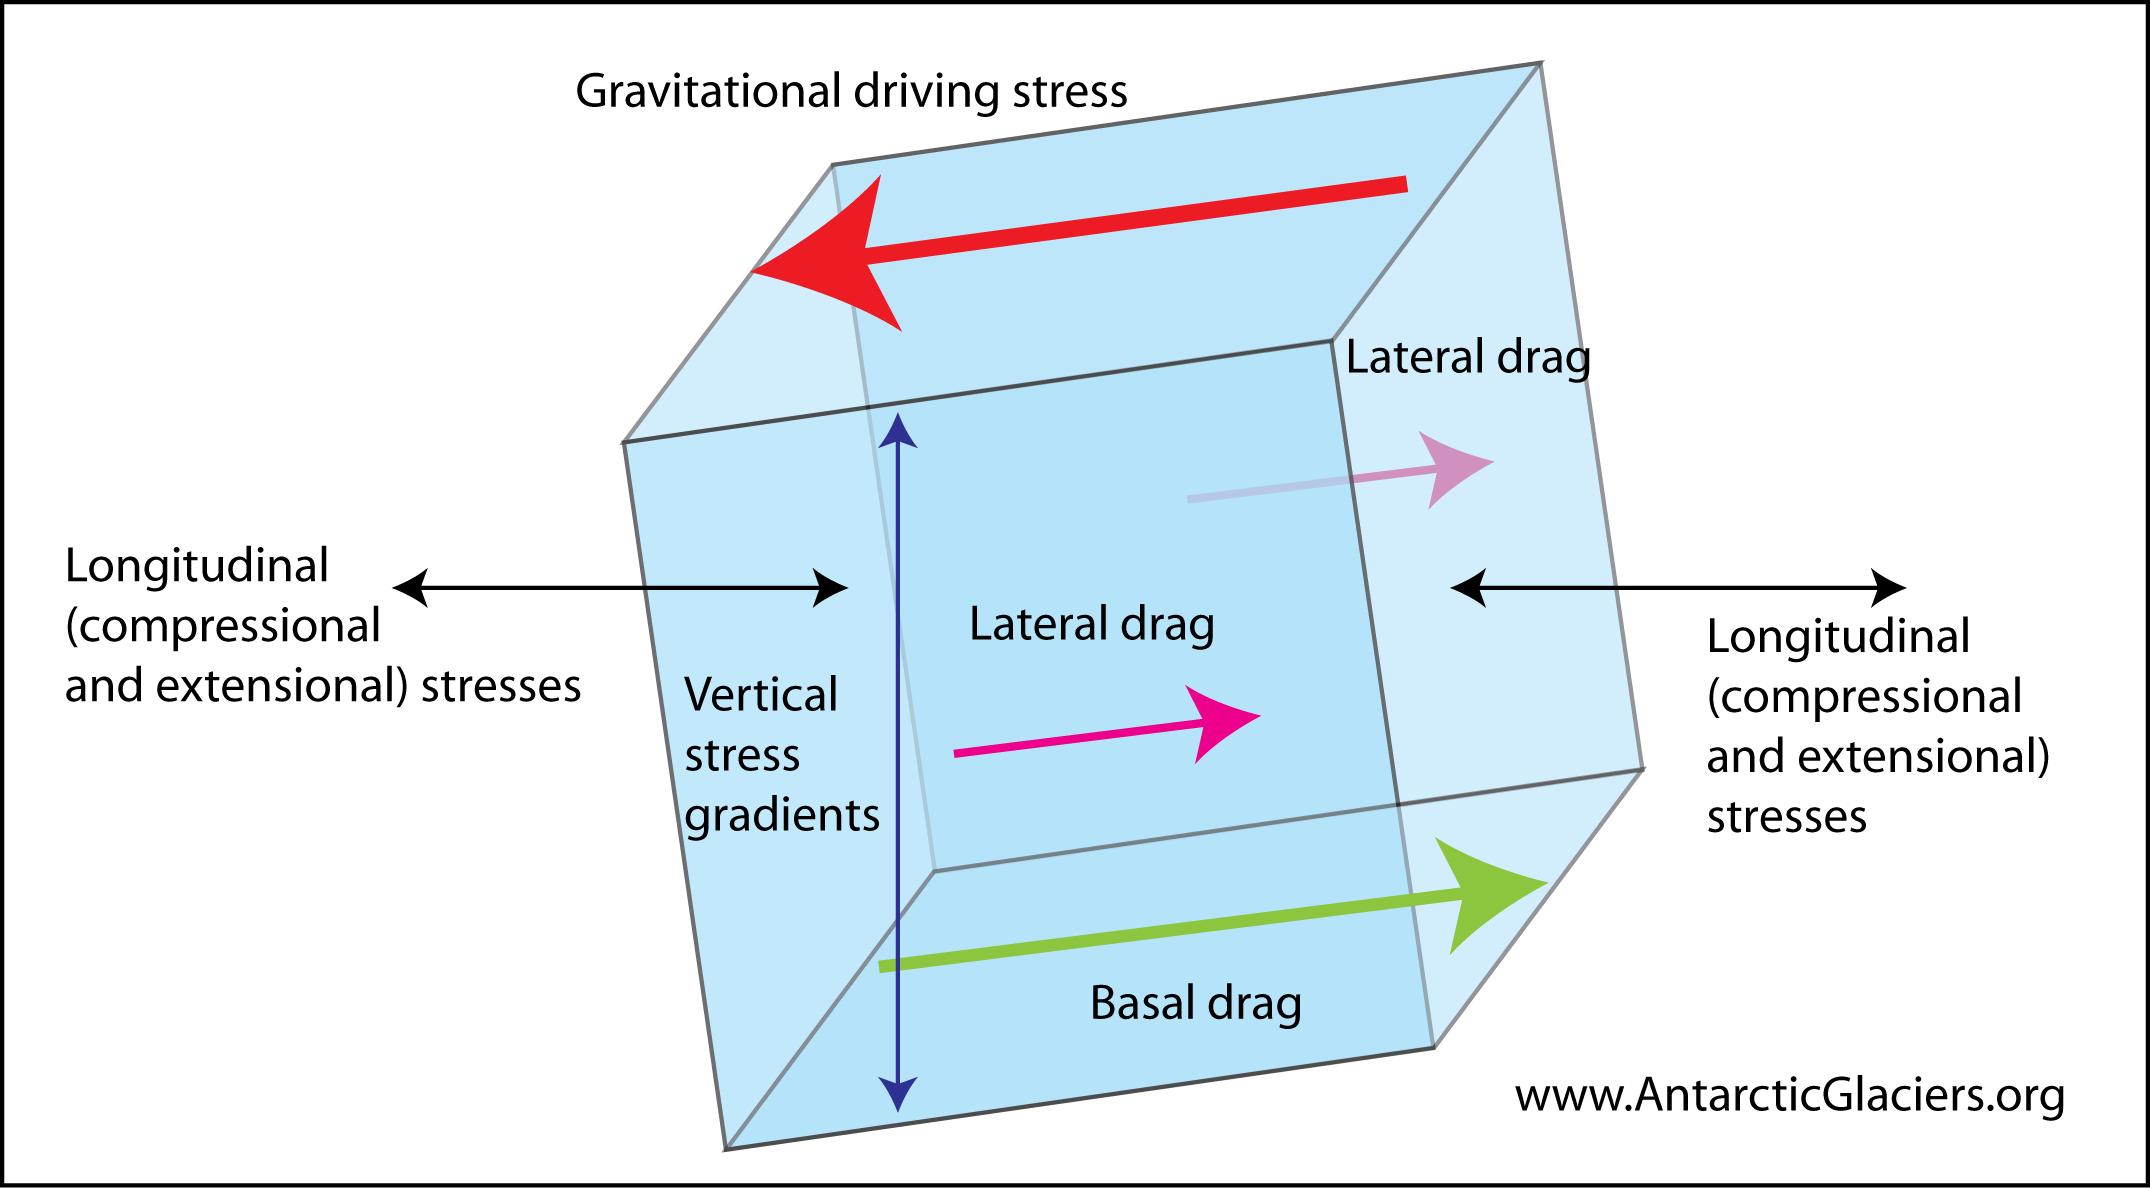
\includegraphics[width=0.7\linewidth]{../fig/nine-stresses.png}
	\caption{Driving and basal stresses on a block of ice. Adapted from AntarticGlaciers.org}
	\label{nine_stresses}
\end{figure}
The SIA is the simplest approximation of the Full Stokes equations. It assumes that basal shear stress of the grounded ice is completely balanced by the gravitational driving stress. It also assumes a small aspect ratio of vertical to horizontal length. (which is appropriate for an ice sheet) and a large ratio of vertical to horizontal stresses. That represents a slow flow in the interior of an ice sheet (blue regions in Figure \ref{velocityglaciar}). Vertical shearing is concentrated close to the bedrock, with almost no vertical shearing near the surface. It also assumes that the longitudinal derivatives of stress, velocity and temperature are small. This is typical of slow ‘sheet flow’ in the interior of ice sheets, and the SIA has been shown to model this well.
Advantages of the SIA include that it is relatively easier to simulate numerically, and for this, to solve computationally, and so well suited to long runs, and it works well on ‘sheet flow’ in the interior of ice sheets. It is well understood, with a long history of use. Disadvantages of the SIA include that it cannot properly represent transition between grounded and floating ice, and does not represent ice shelves or ice streams. It is also not appropriate for complex, local changes, such as at the grounding line; it excludes membrane stresses cross the grounding line.

\begin{figure}[!h]
	\centering
	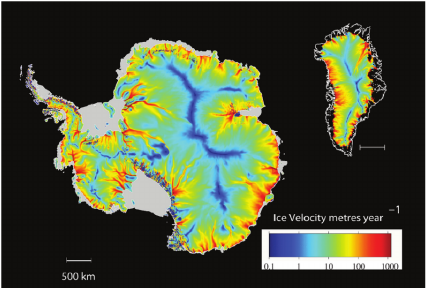
\includegraphics[width=0.7\linewidth]{../fig/velocityglaciar.png}
	\caption{Ice velocities in Antarctica and Greenland topographies, where we can see in red the highest velocity profiles in the glaciers and as a consequence we consider the basal shear stress as 0 and the longitudinal stress dominates, which allows using a Shallow Shelf approximation \cite[]{allison2009ice}.}
	\label{velocityglaciar}
\end{figure}
Figure \ref{velocityglaciar} shows a map of velocities in Antarctica and Greenland topographies. Where this velocity is the highest, the basal shear stress cannot be considered balanced by gravity anymore. Instead, it is taken as 0 and the longitudinal stress dominates. This is the Shallow Shelf approximation, initially developed for ice shelves, but which has been extended to dragging ice streams. It is a 2D vertically integrated model, the ice velocity being depth-averaged.

The factors such as sensitivity, long time intervals, and long distances require careful treatment of the groundline neighbourhood by the numerical method to discretize the model equations \cite[]{cheng2019full}. The most accurate ice model is the Full Stokes (FS) equations \cite[]{cheng2019full}. However, a simplification of these FS equations by integrating into the depth of the ice is the shallow shelf approximation \cite[]{macayeal1989large}. The computational advantage with Shallow Shelf approximation is that the dimension of the problem is reduced by one, it is often used for simulations of the interaction between a grounded ice sheet and a marine ice shelf \cite[]{cheng2019full}. 
In this project, only the Shallow Shelf approximation is made, as this is how future projections of Greenland and Antarctica are done using numerical methods.

\subsection{Grounding line stability}
\label{grounding_line_stability}
There are different variables that play an important role in the dynamics of the glaciers. There is, for example, the grounding line. Its location is still a topic of discussion in the literature surrounding ice sheet dynamics \cite[]{goldberg2018representing}. A long debate on the dynamics of such ice sheets was initiated in the 1970s when \cite[]{weertman1974stability} proposed that a marine ice sheet that lies on an upward-sloping bed is unstable.
The grounding line is the boundary between the ice sheet, sitting on the bedrock, and the floating ice shelves. Ice streams merge with ice shelves in the grounding zone, a zone within which the ice is alternately floating and grounded as tides raise and lower sea level \cite[]{hooke2019principles}. The position and migration of this grounding line controls then the stability of a marine ice sheet.
The marine ice sheet stability hypothesis states that when the bedrock slopes down from the coast towards the interior of the marine ice sheet, which is the case in large parts of West Antarctica, the grounding line is not stable. The figure \ref{grounding_line_instability} shows this concept. The grounding line is initially located on the bedrock sill (left hand side of figure \ref{grounding_line_instability}). This position is stable: the ice flux at the grounding line, which is the amount of ice passing through the grounding line per unit time, matches the total upstream accumulation.
A perturbation is applied at the grounding line, e.g. through the incursion of warm Circumpolar Deep Water (CDW, red arrow in Figure \ref{grounding_line_instability}) below the ice shelf. These warm waters lead to basal melting at the grounding line, ice-shelf thinning and glacier acceleration, resulting in an inland retreat of the grounding line. The grounding line is then located on a bedrock that slopes downward inland (right hand side of figure), i.e. an unstable position where the ice column at the grounding line is thicker than previously. The theory shows that ice flux at the grounding line is strongly dependent on ice thickness there \cite[]{weertman1974stability, schoof2007ice}, so a thicker ice leads to higher ice flux. Then, the grounding line is forced to retreat since the ice flux at the grounding line is higher than the upstream accumulation. This is a positive feedback and the retreat only stops once a new stable position is reached (e.g. a bedrock high), where both ice flux at the grounding line and upstream accumulation match.

\begin{figure}[!h]
	\centering
	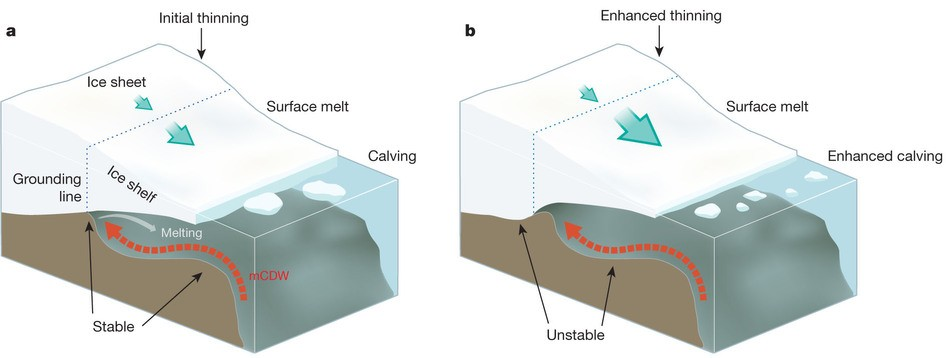
\includegraphics[width=0.7\linewidth]{../fig/Grounding_line.png}
	\caption{Schematic representation of the marine ice sheet instability with an initial stable grounding line position (left hand side) and unstable grounding line position after the incursion of warm circumpolar deep water below the ice shelf. Adapted from \cite{hanna2013white}.}
	\label{grounding_line_instability}
\end{figure}

\cite{weertman1974stability} was the first one to propose a model to handle the behaviour of the glacier dynamics at the grounding line vicinity. Figure \ref{weertman} shows a symmetric two-dimensional ice-sheet. The author proposed that a considerable insight is often gained in problems of glacier mechanics by making the assumption that ice is a perfect plastic solid. Such is the case  with the ice sheet-ice shelf transition zone, namely, grounding zone. For an ice shelf with a positive accumulation, this simplified ice shelf must have a thickness $h_{1p}$ equal to:

\begin{equation}
	h_{1p}=\frac{\tau_0}{\Delta \rho g};
\end{equation}

\begin{figure}[!h]
	\centering
	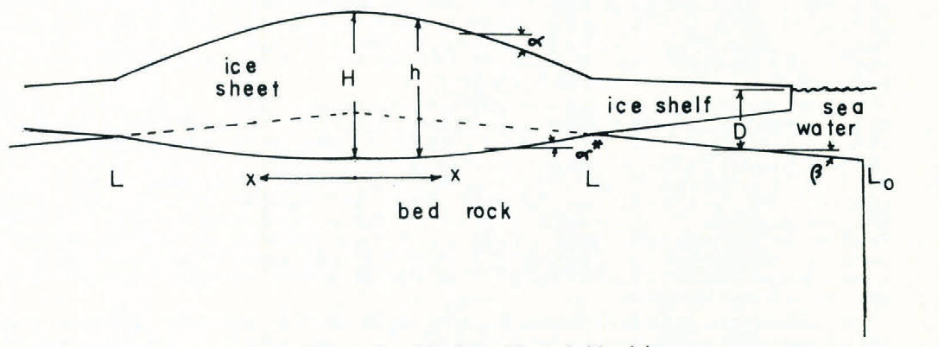
\includegraphics[width=0.7\linewidth]{../fig/Weertman.png}
	\caption{Cross section of ice sheet with attached ice shelves. Adapted from \cite{weertman1974stability}.}
	\label{weertman}
\end{figure}

If the thickness of an ice shelf were greater than $h_{1p}$ it would strain at an infinite rate until its thickness were reduced to the value $h_{1p}$. If the thickness were smaller than $h_{1p}$, the ice shelf would not creep but its thickness would increase in time because of the positive accumulation rate until it reached the value $h_{1p}$. By similar reasoning the basal shear stress of the ice sheet must take on the value $\tau=\tau_0$. The ice sheet profile thus is found by integrating the equation:

\begin{equation}
	\rho gh\alpha=\tau_0;
\end{equation}

where:

\begin{equation}
	\alpha=-(I-\frac{\rho}{\rho_r})\frac{dh}{dx}+\beta(I-\frac{\rho_w}{\rho_r});
\end{equation}

If the ice sheet bed were flat before the ice sheet was placed on it ($\beta=0$) the solution of the equations is:

\begin{equation}
	h^2=H^2-\frac{2\tau_0x}{\rho g(I-\frac{\rho}{\rho_r})}= h^2+\frac{2\tau_0(L-x)}{\rho g(I-\frac{\rho}{\rho_r})};
\end{equation}

Where $H$ given by:
\begin{equation}
	H^2=h^2+\frac{2\tau_0L}{\rho g(I-\frac{\rho}{\rho_r})};
\end{equation}

is the thickness of the ice sheet at the center $x=0$ and $h_2$ is the thickness of the ice sheet at its edges ($x=L$). Because the ice sheet is afloat and its edges the thickness $h_2$ is equal to:

\begin{equation}
	h_2=(\frac{\rho_w}{\rho})D(L);
\end{equation}

When $\beta=0$ the ice sheet profile is given by:

\begin{equation}
	(H-h)-(\frac{I}{A})ln[\frac{AH-I}{Ah-I}]=\frac{\tau_0 Ax}{\rho g(I-\frac{\rho}{\rho_r})};
\end{equation} 

Where:

\begin{equation}
	A=\frac{\beta \rho g}{\tau_0}(I-\frac{\rho_w}{\rho_r});
\end{equation}
The value of H is found by setting $h=h_2$ at $x=L$.

For the condition at the grounding line position, $x=L$, the thickness of the ice shelf, $h=h_2$ is such that the ice sheet is afloat. The ice shelf is also afloat. Thus, the thickness of the ice shelf, $h=h_{1p}$, must satisfy the condition:

\begin{equation}
	h_{1p}<h_2;
\end{equation}

Supposing that $h_{1p}$ was appreciably smaller than $h_2$, situation illustrated in figure \ref{Instability_condition}. The ice sheet is shopped off essentially at $x=L$. The effect of this truncation at the edge of the ice sheet is to cause a large longitudinal tensile stress to be set up in the ice sheet near its edge. The magnitude of this tensile stress must be of the same order as that of the stress existing in an ice shelf of thickness $h_2$. Since $h_2>>h_{1p}$ the strain rate near its edge is infinite if ice is a perfect plastic solid \cite[]{weertman1974stability}. Therefore it is not possible to have $h_2>>h_{1p}$ and have the ice sheet and the ice shelves in a steady state condition. So, it is concluded that the grounding line position will be stable if:
\begin{equation}
	h_2 \approx h_{1p};
\end{equation}

\begin{figure}[!h]
	\centering
	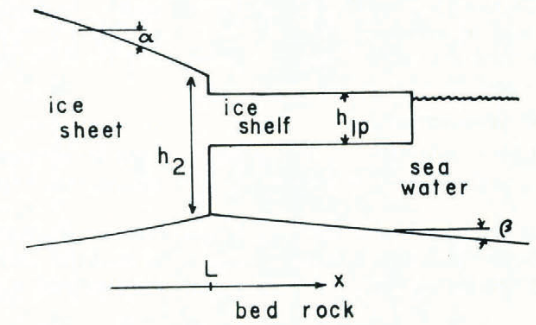
\includegraphics[width=0.7\linewidth]{../fig/H2.png}
	\caption{Grounding line position as the junction between ice shelf and ice sheet. No restriction on thickness of ice sheet at x = L. Adapted from \cite{weertman1974stability}.}
	\label{Instability_condition}
\end{figure}

Recently, the instability hypothesis has been strongly reinforced, based on a boundary-layer theory due to \cite{schoof2007ice}. Moreover, \cite{vieli2005assessing} showed the poor ability of marine ice-sheet models to give consistent prognostic results and, more particularly, they highlighted the influence of the grid size on model results. One of their main conclusions was that no reliable model was able to predict grounding line dynamics at the time of their study.

There is a need to improve marine ice-sheets models in order to corroborate recent theoretical predictions and to obtain confident simulations of the grounding line dynamics. \cite{durand2009marine} proposed a full-Stokes solution of the ice-sheet/ice-shelf transition. This approach has been built on literature dealing with the coupling between a grounded ice sheet and a floating ice shelf and identifying this transition zone as a crucial control of the marine ice sheet dynamics, like the studies carried out by \cite{weertman1974stability}, \cite{van1985response}, \cite{schoof2007ice}, and \cite{schoof2007marine}. Also, \cite{chugunov1996modelling} presented a model for the behavior of a marine glacier and ice-sheet-ice-shelf transition zone based on asymptotic analysis, which involves breaking down the equations into simpler components and analyzing their behavior as certain variables approach infinity or zero, to derive a set of simplified equations that can be used to predict the behavior of the glacier and ice-sheet-ice-shelf transition zone. \cite{hindmarsh1996stability} presents a mathematical model of ice rise stability, which takes into account the effects of ice flow, ice shelf melt, and ocean circulation. He uses this model to analyze the stability of several ice rises and uncoupled marine ice sheets in Antarctica, finding that some of these features may be more stable than previously thought. On the other hand, \cite{vieli2005assessing} evaluate the ability of numerical ice sheet models to simulate grounding line migration. They concluded that while numerical ice sheet models have made significant progress in simulating grounding line migration, there is still much work to be done to improve their accuracy and reliability.

\cite{durand2009full} showed, using the finite element code Elmer/Ice, that the full-Stokes modeling of the ice-sheet/ice-shelf transition gives a consistent prediction of grounding-line migration. However, their approach is highly sensitive to the chosen mesh resolution. For a grid size smaller than $5 km$ in the grounding-line vicinity, predictions start to be consistent. For any finer resolution than $5 km$, the steady-state grounding-line position is the same (6km is the standard deviation). If a sub-grid refinement of 200m in the vicinity of the grounding line is applied the steady-state position is stable.

As a more general conclution from the theory, it confirms the proposition made by \cite{weertman1974stability} that the ice flux is a function of ice thickness at the grounding line in the case of a 2-D flow problem with no lateral shearing in ice shelf, as it is the case for a shallow shelf approximation of the full stokes model. For this reason, in order to study and test the behavior of the impact of the mesh resolution on the migration of the grounding line position, idealized systems are studied and, based on the results that are obtained from these idealized cases, the hypothesis, models, and numerical methods used to solve the problems may be improved. The main focus of the experiments proposed in this project is to test the influence of the mesh resolution on the prediction of the grounding line position using a numerical model to solve a shallow shelf approximation of the governing equations of ice flow. 

\section{Numerical methods}
\label{Numerical_methods}
Analytical solutions to problems of glacier flows could be obtained only when the problems are quite simple \cite{hooke2019principles}. Thus, two numerical methods are the most used in modelling: the finite difference methods and the finite element method. More recently, the finite-volume method has been deployed, and researchers are experimenting with less physically-based techniques \cite{hooke2019principles}.

Finite-difference modeling is basically an extension of numerical integration. The defining characteristic of the finite-difference method is that gradients in a parameter are approximated by obtaining values of the parameter at grid points and dividing by the distance between the grid points. Finite-difference techniques can also be used to integrate the momentum equation, but simplified versions of the momentum equation can be integrated analytically.

The finite element method is another way of obtaining an approximate solution to
the governing equations. In finite-element as in finite-difference models, the
domain of interest is broken up into a large number of small elements. In early
applications of finite-element models to glaciological problems the elements were
quadrilaterals, but commercial packages now in use commonly have higher-order
element geometries. The corners of elements are called nodes. Unlike finite-
difference models, in a finite-element model there is no advantage in making all
of the elements rectangular and the same size \cite{hooke2019principles}.

In finite-element calculations, use is made of the fact
that the relevant differential equations can be expressed in a form consisting of a sum of integrals. A solution method, called the method of weighted residuals, then guarantees that the resulting approximate solution will be the best possible solution mathematically obtainable with a given element configuration. While initially more complicated to understand, finite-element formulations have been shown to be generally numerically more stable than finite-difference formulations \cite{hooke2019principles}. Furthermore, element shapes can be adjusted to conform to boundaries that would be awkward to model with rectangular elements Finally, element size can be reduced in areas of low gradients and increased in areas of high gradients, as near the bed , thus increasing accuracy without increasing computation time. Complex, non-uniform, and variable boundary conditions are also easier to include in finite-element models.

Once a domain is discretized, stress or velocity conditions are specified at boundary nodes and equations are written relating stresses and velocities at interior nodes to each other, to the mean stress in the element, and to the stresses or velocities at the boundaries. As usual, the basic equations being solved are those for conservation of momentum, mass, and energy. Although the number of equations to be solved simultaneously is large, the number of unknowns in each equation is small, so efficient routines for solving sparse matrices can be used. Owing to the non-linearity of the flow law, the set of equations is non-linear and an iterative solution is necessary. A trial solution is given initially, and this is corrected to obtain an improved solution at each iteration. For these reasons, the finite element method is commonly the most used to model the stokes equations and approximations derived from these in glacier dynamics. 

\section{Numerical model}
\label{Numerical_model}
\subsection{The Elmer/Ice finite element method}

\begin{figure}[!h]
	\centering
	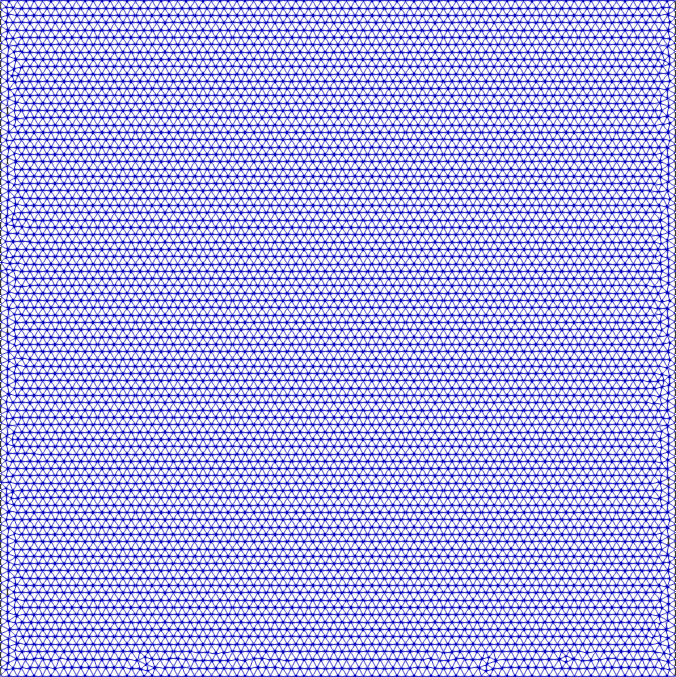
\includegraphics[width=0.45\linewidth]{../fig/non_structured_grid_10km.png}
	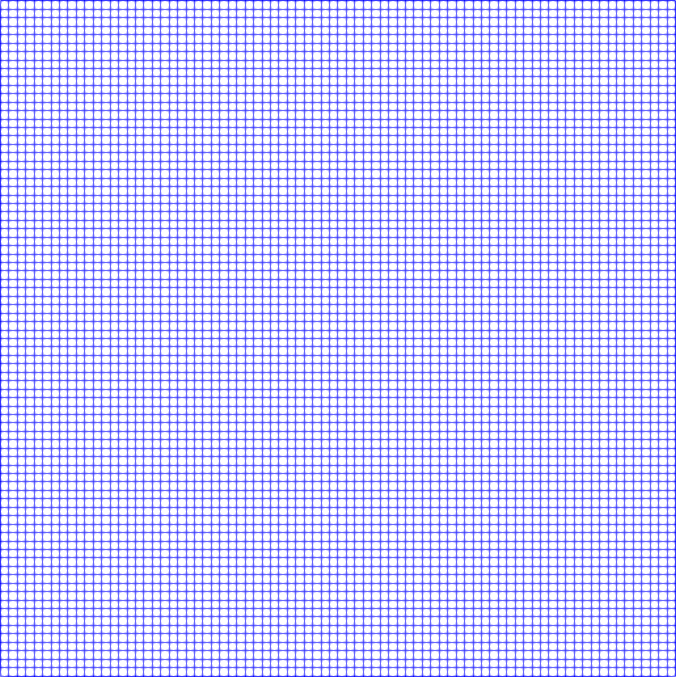
\includegraphics[width=0.45\linewidth]{../fig/regular_grid_10km.png}
	\caption{a) 10km resolution non-structured mesh used in Elmer/Ice. b) Regular structured mesh for 10km resolution.}
	\label{meshes}
\end{figure}

Most of the time analytical solutions are challenging or even impossible to obtain. In order to model ice sheets, both the finite difference method (FDM) and the finite element method (FEM) are used. The finite difference method consists in converting ordinary and partial differential equations into a system of linear equations by approximating derivatives as finite differences. Elmer/Ice, on the other hand, uses the finite element method.

The ice sheet/ice flow model Elmer/Ice includes developments related to glaciological problems and a large number of dedicated solvers and user functions that solve the Full-Stokes equations for various ice rheologies (classical, Glenn's flow law, anisotropic laws, and porous compressible firns/snow law). It includes solvers for the classical asymptotical expansions of the Stokes equations, namely the shallow ice approximation and the shallow and shallow shelf approximation (SSA). All these equations can be solved diagnostically or transiently, allowing the displacement of the boundaries.

Elmer/Ice considers a continuum as an assembly of non-overlapping elements forming the same geometry, which makes the modeling of complex geometries possible. Each element is made of at least two points, which are applied to the forces and computed the displacements. To solve the equations, Elmer/Ice uses subroutines or solvers. Each equation corresponds to one solver to be referenced in the input file, together with the different parameters of the problem. They each compute the evolution of given variables, such as the ice thickness or the velocity, to give at each time step a picture of the flow. All combined, it allows us to visualize the evolution of the flow through time.

As mentioned before, the simulations using Elmer/Ice use unstructured meshes, as shown in the left-hand side of figure \ref{meshes} for a 10km resolution mesh. This is very helpful in terms of simulating complex geometries, for example, the thule configuration.


However, once the simulation is done and to better interpret the results obtained, it is needed to build a structured mesh, because it is ideal for these time-domain simulations this it can  easily identified elements and nodes when plotting time-dependent or spacial-dependent graphics. In this case, the objective of interest will be the spacial behaviour or dynamic of the glacier since the interest is to analyse the position of the grounding line after the steady state is reached. To build the structured mesh, an interpolation made from the unstructured mesh values of the nodes is performed, namely an interpolation per each node of the value of the variables of interest with the values of these same variables in the non-structured mesh. This way the position where the node is, and the spacial dependent variables can be plot; for example, the velocity components as a function of the horizontal position. 

\section{Numerical parameters}
\label{Numerical_parameters}
\subsection{Physical parameters}
Table \ref{Physical constants} shows the physical parameters that were set up for the experiment by the CalvingMIP project. This are the parameters that are used in the model to solve the flow equations:

These parameters were modified by the CalvingMIP intercomparisson project after the current project was proposed. The water density and the time equivalence from year to seconds was changed from 1030 kg/m$^3$ to 1028 kg/m$^3$ and from 365.2422 days in a year to 31556926 s in a year, respectively. All the rest of the parameters remained the same as listed in table \ref{Physical constants}.

For the computation of $u_b=2$, we used the Weertman style sliding law:

\begin{equation}
	u_b = C\tau _b^m
\end{equation}
where C is the basal slipperiness and $\tau _b$ is the basal shear stress.
In order to enter these values into the Elmer/Ice code, we need to convert all units to Elmer/Ice units, namely: MPa, meter, and years. It means that all units that are derivated from time in seconds, must be converted to time in years using the time equivalence proposed in the project and all units or values expressed in terms of KPa must be multiplied by a factor of $10^{-3}$ to be converted to MPa.
Also, to compute the basal sliding velocity $u_b$, Elmer/Ice uses the term $\beta$ that is related to $u_b$ by:
\begin{equation}
	\tau = \beta u_b^{\frac{1}{m}}
\end{equation}
So, we have:
\begin{equation}
	u_b = (\frac{\tau}{\beta})^m;
\end{equation}
\begin{equation}
	u_b = \frac{1}{\beta^m} \tau^m
\end{equation}
Using the notation from equation (1), we can say that $C=  \frac{1}{\beta^m}$. So, we can compute $\beta$ as:
\begin{equation}
	\beta=(\frac{1}{C})^{\frac{1}{3}}
\end{equation}
If we replace C by its value given in table \ref{Physical constants}, we get $\beta$= 10$^4$Pa m$^{\frac{-1}{3}} a^{\frac{1}{3}}$ which converted to MPa will give us a value of 10.

\begin{table}[!h]
	\begin{center}
		\caption{Physical parameters}
		\label{Physical constants}
		\begin{tabular}{|l|l|l|}
			\hline
			Variable          & Description                 & Units           \\ \hline
			$g=9.81$         & Gravitational acceleration  & ms$^{-2}$         \\ \hline
			$a_s=0.3$       & Surface mass balance (SMB)  & ma$^{-1}$         \\ \hline
			$a_b=0$             & Basal mass balance (BMB)    &   ma$^{-1}$         \\ \hline
			$\rho i=917$        & Ice density                 & kg m$^{-3}$       \\ \hline
			$\rho w=1028$      & Sea water density           & kg m$^{-3}$       \\ \hline
			$A= 2.9377$x$10^{-9}$ & Ice rate factor             & KPa$^{-3}$a$^{-1}$  \\ \hline
			$n=3$               & Flow law stress exponent    &  Dimensionless               \\ \hline
			$C=0.001$           & basal slipperiness          & ma$^{-1}$KPa$^{-3}$ \\ \hline
			$m=3$               & Sliding law stress exponent &   Dimensionless              \\ \hline
			$s2a=31556926$     & Seconds in a year           & s         \\ \hline
		\end{tabular}
	\end{center}
\end{table}

\subsection{Numerical variables}
The numerical resolution will be our variable parameter, which we will vary from 10 km, 5 km, 2 km, 1 km.
\subsection{External forcing}
We will assume that the forces acting are gravity ($g=9.81 m/s^2$), which is translated to the weight of the ice sheet and the flotation force of this in the ocean water, as well as the ice friction with the bedrock, and the basal stress.
\subsection{Initial condition}
The simulation departs from no ice configuration, from a topography with no ice, namely $h_0 = 0$. However, the Elmer/Ice numerical method code, that will be used for these experiments, uses a notation where at least a minimum value should be enter in order to avoid convergence problems, so a very small value of $h_0 = 1$m is introduced as initial ice thickness. 
\subsection{Time step}
The Courant-Friedrichs-Lewy (CFL) condition is a necessary condition to solve numerical partial differential equations. It states that the distance a variable travels between two-time steps must be smaller than the distance between two points of the mesh \cite[]{courant1967partial}. It is needed that:
\begin{equation}
	C=\frac{u\Delta t}{\Delta x}<C_{max};
\end{equation}
With C the courant number, $u$ the magnitude of the velocity, $\Delta t$ the time step, $\Delta x$ the horizontal resolution, and Cmax = 1. This implies then, for a given mesh:
\begin{equation}
	\Delta t < \frac{\Delta x}{u};
\end{equation}
This is a safe approximation. Cmax then has to be estimated by running different parameters in the simulation and seeing if it converges or not. In order to satisfy the CFL condition, a good starting point is 1 year, since it works properly and converges even for a resolution of 1km.
\subsection{Boundary conditions}
Boundary conditions are needed in order to solve differential equations. It will be assumed that:
\begin{itemize}
	\item The bedrock is impermeable (The vertical component of the ice flow velocity is 0):
	\begin{equation}
		v = 0
	\end{equation}
	\item The flow follows the Weertman friction law:
	\begin{equation}
		u_b = C\tau_b^m
	\end{equation}
	\item Mass accumulation is a constant parameter.
	\item The simulation will be performed on a quarter of the domain since the geometry of the topography is symmetric, which allows having free slip boundary conditions at the left and downsides of the topography, and open boundary conditions at the right and top sides of the domain. 
\end{itemize}

\section{System and experiment set-up}
\label{Systems}
\subsection{Cone domain}

The formation of CalvingMIP is being undertaken as part of PROTECT, an EU funded project to "assess and project changes in the land-based cryosphere, with fully quantified uncertainties, in order to produce robust global, regional and local projections of SLR on a range of timescales". These efforts are set to culminate in a world-wide model intercomparison project on ice damage and calving, comparing the novel routines to standard approaches/calving laws, leading to recommendations for improved calving laws in ice sheet models.

The idealised experimental domain comprise a simple, symmetrically circular domain. This first idealized model consists of a circular bedrock configuration (Figure \ref{circular_topo_top}) given by:
\begin{equation}
	\theta=arctan2(y,x);
\end{equation}
\begin{equation}
	I=r-cos(2\theta)\frac{r}{2}
\end{equation}
\begin{equation}
	Bed_0=Bc-(Bc-BI)\frac{|x^2+y^2|}{r^2};
\end{equation}
Where r=800x10$^3 m$, Bc=0.9 x 10$^3 m$, and BI=-2 x 10$^3 m$. 
\begin{figure}[!h]
	\centering
	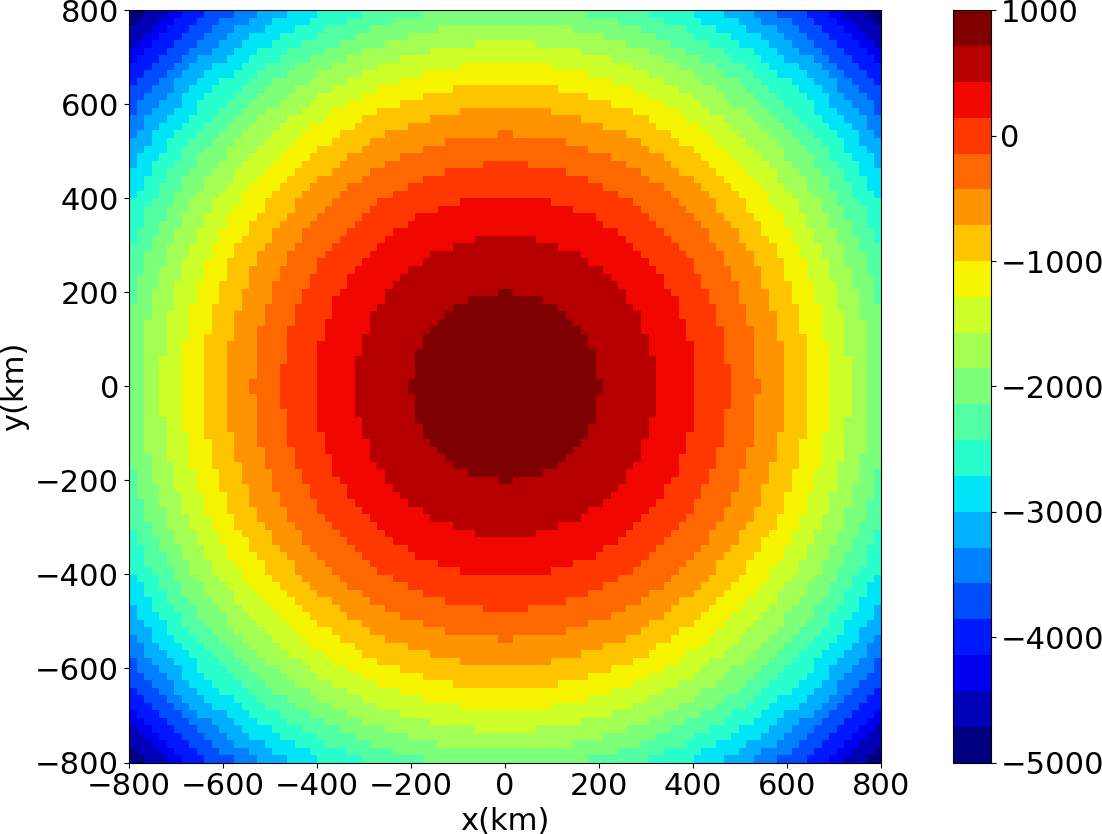
\includegraphics[width=0.45\linewidth]{../fig/circular_topo_top.png}
	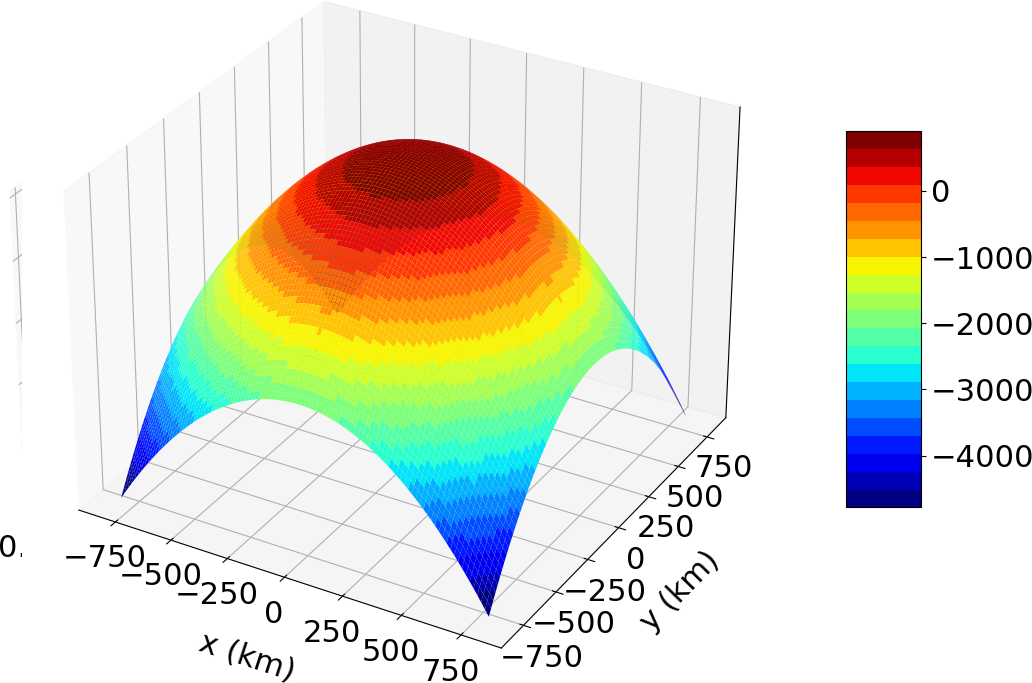
\includegraphics[width=0.45\linewidth]{../fig/circular_topo_jet}
	\caption{Circular bedrock topography. On the left side top view and on the right side, lateral view.}
	\label{circular_topo_top}
\end{figure}

This experiment is intended to provide initial conditions for future calving experiments using the circular domain as well as other test participating models capability to maintain a steady unchanging calving front. To this end, the idea is to spin up an ice sheet in the circular domain from no initial ice thickness to an ice sheet in steady state with a calving front located in a circular with radius 800 km from the center of the domain. The calving front position should be maintained by imposing a calving rate that is equal and opposite to the ice velocity at the calving front, resulting in a calving front position that does not move.
Note that, in this particular experiment, the interest does not consist in the exact means by which the steady state condition is achieved but instead the experiment is concerned with the final steady state. 
Also, due to the symmetry of the domain with respect to both axis, the domain can be reduced to a quarter.

\begin{figure}[!h]
	\centering
	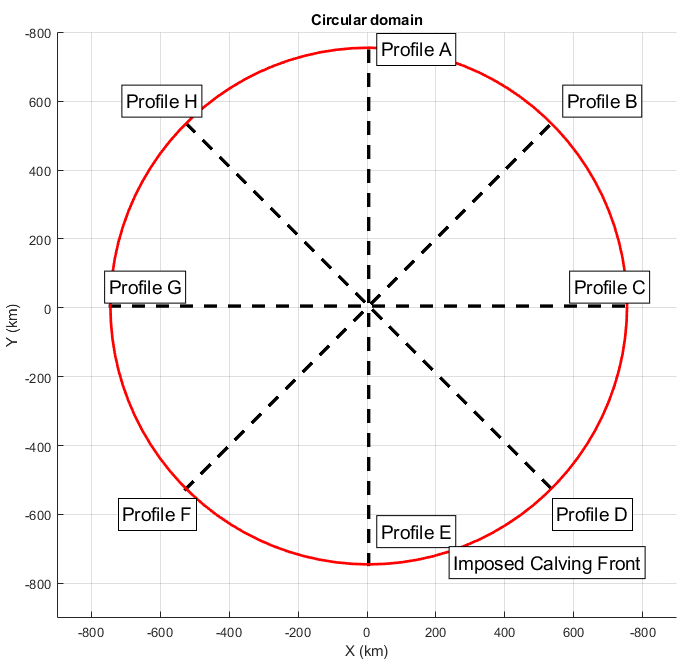
\includegraphics[width=0.7\linewidth]{../fig/cone.png}
	\caption{Circular domain experimental profiles as well as the initial imposed calving front position. Adapted from CalvingMIP inter-comparison project.}
	\label{cone_profile}
\end{figure}

\subsection{Thule domain}
The Thule bedrock configuration is shown in Figure \ref{Thule_3D} and is given by:
\begin{equation}
	\theta=arctan2(y,x);
\end{equation}
\begin{equation}
	I=r-cos(2\theta)\frac{r}{2};
\end{equation}
\begin{equation}
	Bed_0=Bc-(Bc-BI)\frac{|x^2+y^2}{r^2};
\end{equation}
\begin{equation}
	Bed=Bacos(3\pi\frac{\sqrt[2]{x^2+y^2}}{I})+Bed_0;
\end{equation}
With r=800 x 10$^3 m$, Bc=0,9 x 10$^3 m$, BI=-2 x 10$^3 m$, and Ba=1.1 x 10$^3 m$.
\begin{figure}[!h]
	\centering
	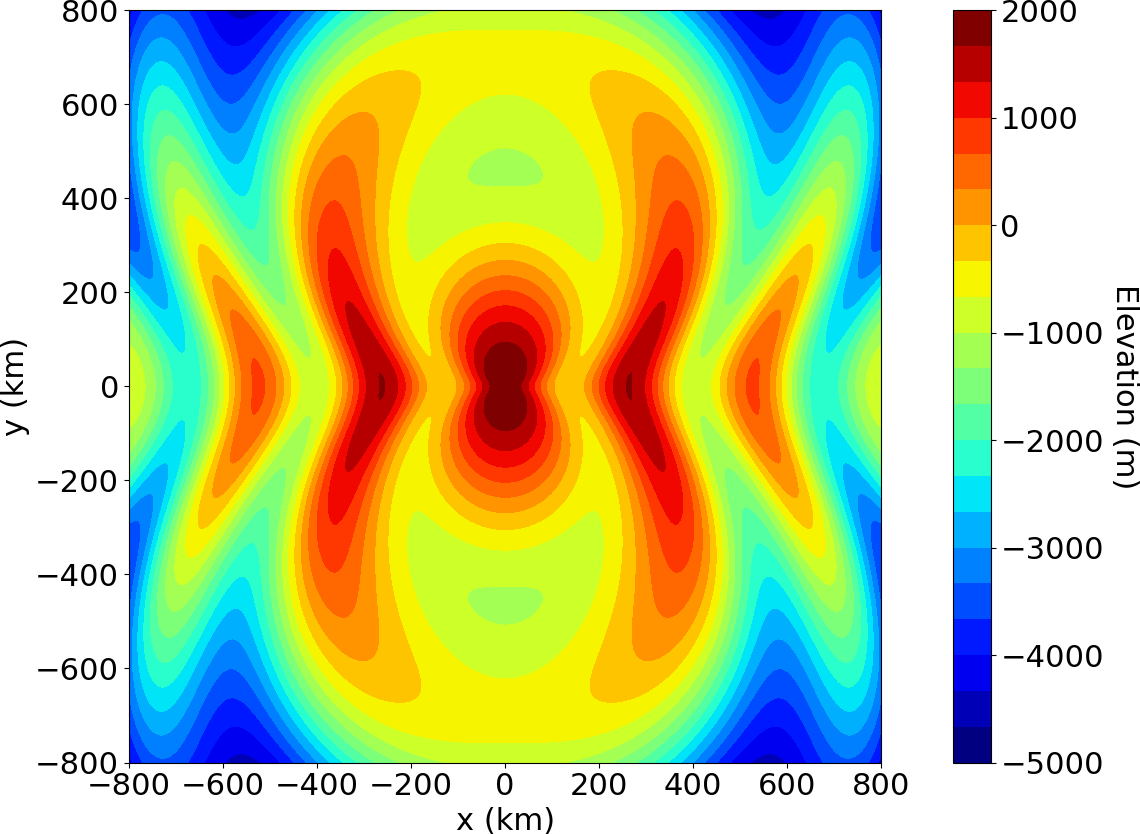
\includegraphics[width=0.45\linewidth]{../fig/Thule_2D}
	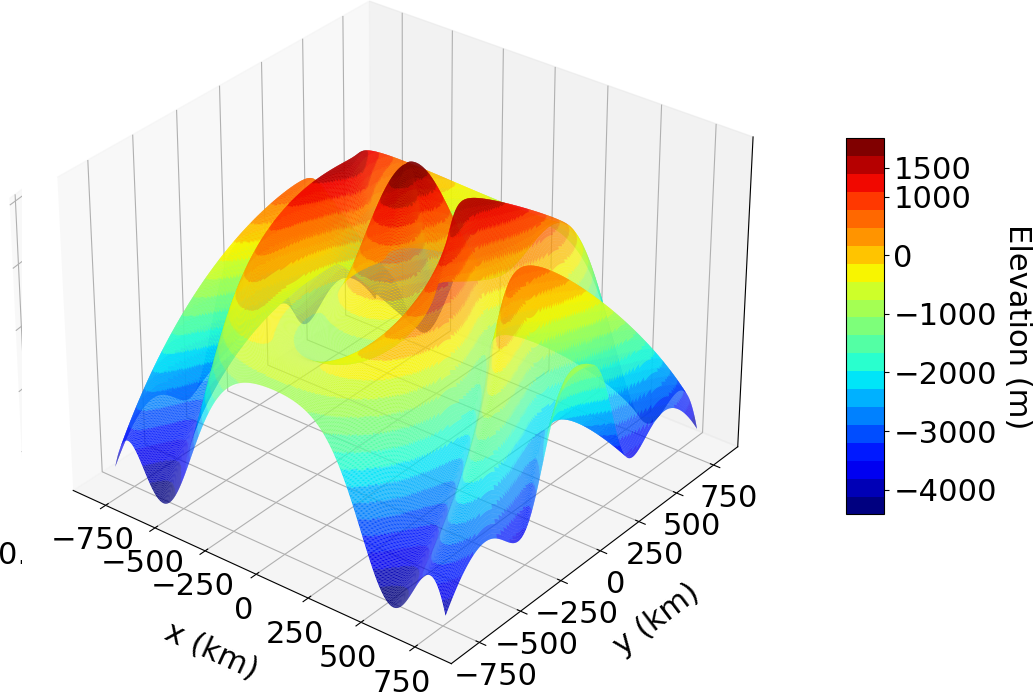
\includegraphics[width=0.45\linewidth]{../fig/Thule_3D}
	\caption{Thule bedrock topography 3D. On the left side the top view, and on the right side a lateral view.}
	\label{Thule_3D}
\end{figure}
\begin{figure}[!h]
	\centering
	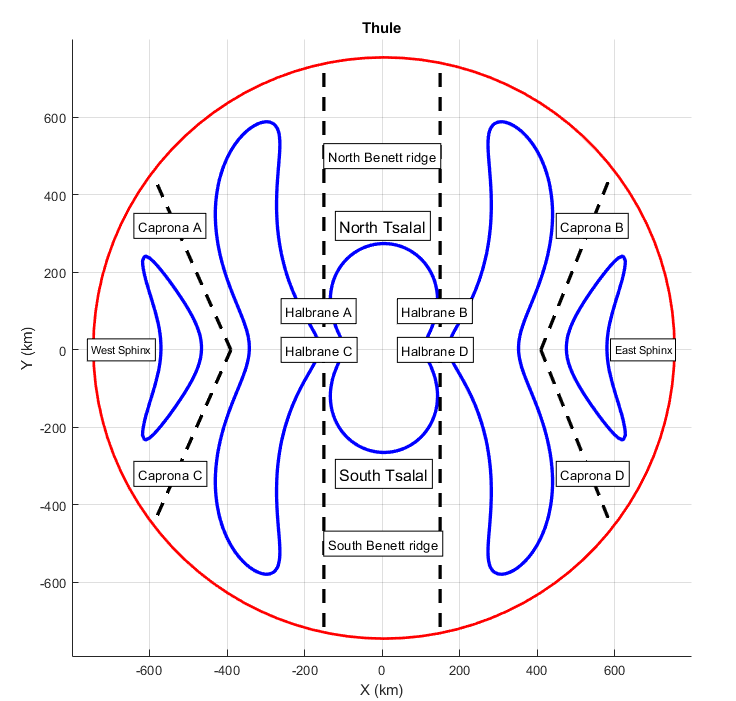
\includegraphics[width=0.7\linewidth]{../fig/thule.png}
	\caption{Thule domain experimental profiles as well as the initial imposed calving front position. Adapted from CalvinMIP inter-comparison project.}
	\label{thule_profile}
\end{figure}
The second experiment is intended to provide initial conditions for future calving experiments using the Thule domain as well as test participating models capability to maintain a steady unchanging calving front. To this end, the idea is also to spin up an ice sheet in the Thule domain from no initial ice thickness to an ice sheet in steady state with a calving front located in a circul with radius 800 km from the centre of the domain. The calving front position should be maintained by imposing a calving rate that is equal and opposite to the ice velocity at the calving front, resulting in a calving front position that does not move. 

For the Thule domain it is convienient to name some geographical features that arise due to the underlying bedrock bathymetrym as such they are defined the North and South Tsalal, East and West Sphinx and Caprona A, B, C and D ice shelves, as observed in figure \ref{thule_profile}. They are also defined the North and South Benett ridges as being the ridges in bedrock bathymetry located under the North and South Tsalal ice shelves respectively. Finally,  Halbrane A and B ice streams are defined as those feeding into the North Tsalal ice shelf whilst Halbrane C and D feed into the South Tsalal ice shelf.

For the quarter of the domain, the experiment will be performed along Caprona B and Halbrane B profiles due to the symmetry of the domain.

Both experiments are performed modeling the SSA approximation of the stokes equations until the steady state is reached. Once the variation in time is 0 (or very small) the convergence of the system is concluded and the system has reached the final steady state. For both experiments, the grounding line position along the defined proposed profiles is calculated. For this, a function that can be denominated grounding line needs to be created, and this function is defined as the product of the bedrock position and a grounding mask. This grounded mask is a step function created, which a value of -1 is assigned to the grounded ice, and 1 to the part of the ice that is no longer in contact with the bedrock, namely:

\[ Groundedmask = \begin{cases} 
	-1 & bedrock = z_b \\
	1 & z_b \leq bedrock   
\end{cases}
\]

Using this mask, the grounding line function is defined as the negative product of this mask and the bedrock (the negative sign is only implemented for convention). From the fact that this grounding line function is an increasing function, it must have an unique maximum, namely, the point where the function changes sign. This maximum means the point where $z_b$ is no longer equal to bedrock position, so starting from this point, the lower part of the ice sheet is not grounded any more. This maximum value of the grounding line function corresponds, physically, to the point where the grounding line or zone is along an x-profile. Knowing this point, the distance from the origin of our coordinate system to that point can be computed, knowing the x and y coordinates of this point, as the norm if this vector, this distance determines the grounding line position, in meters, along an x axis. The results will be calculated in two parts: along three profiles A,B and C for the quarter of the domain, and along all the profiles from A to H for the domain complete, in the case of the Cone domain experiment. For the thule experiment, in the first part the grounding line position along Caprona B and Halbrane B needs to be calculated for the quarter domain, and then along all Capronas and Halbranes profiles for the complete domain. For both cases, per each resolution the mean, maximum and minimum value of the grounding line position will be calculated.

\section{Results}
\label{Results}
\subsection{Cone configuration}

Using the settings for the experiment described in the previous sections, different simulations were driven varying the resolution mesh from 10km, 5km, 2km and 1km. Steady state was reached and the corresponding ice sheet-ice and ice shelf surface profiles are plotted in figure \ref{Cone_scheme}. In this figure it is highlighted the quarter of the domain in figure \ref{Schematic_Cone} and its three profiles A,B,C since, as mentioned before, both simulations for the domain complete and the quarter domain were run to compare the results. The point or zone where the lower part of the ice sheet stops being in contact with the bedrock is the grounding line, along each profile (figure \ref{Profiles_cone}).

\begin{figure}
	\centering
	\begin{subfigure}{.5\textwidth}
		\centering
		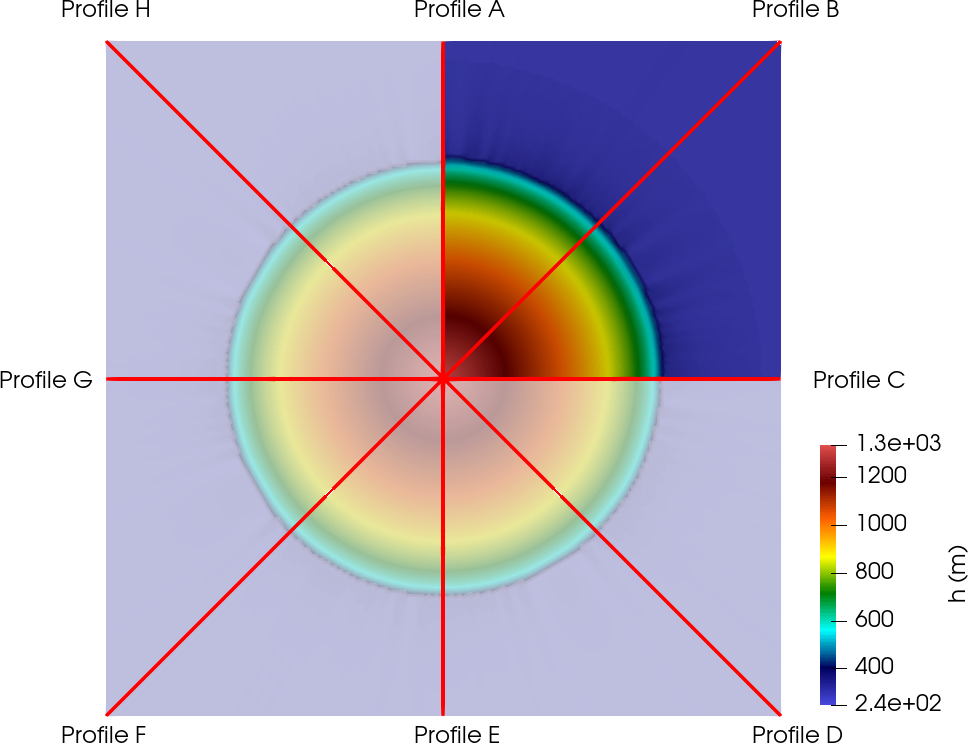
\includegraphics[width=0.99\linewidth]{../fig/Profiles_Cone_combined_domains.png}
		\caption{Profiles for Cone circular domain}
		\label{Schematic_Cone}
	\end{subfigure}%
	\begin{subfigure}{.5\textwidth}
		\centering
		\includegraphics[width=0.99\linewidth]{../fig/Profiles_Cone_domain_sin_fondo.png}
		\caption{Ice thickess per profile}
		\label{Profiles_cone}
	\end{subfigure}
	\caption{Schematic representation of the circular domain ice sheet showing the ice thickness results along the profiles proposed.}
	\label{Cone_scheme}
\end{figure}

The figure \ref{Volume_CONE_VS_TIME_VS_NODES} shows the evolution in time for the volume and the ice thickness per each resolution, showing the convergence of the simulation (50000 years for the 10km resolution, 3000 years for 5 and 2 km resolution, and around 1000 years for the 1km resolution). It is important to remark that for convenience purposes in these figures the time axis for the 10 km resolution was divided by 10 to be in the same scale with the results for the other resolutions. It can be observed that the ice thickness increases as the resolution increases. For this reason, the volume of the ice sheet increases as the mesh resolution increases, as it can be observed in figure \ref{VOLUME_CONE_VS_TIME}. This figure shows the convergence of the volume after certain amount of simulation time per each resolution, showing that a steady state was reached. This behaviour is expected since the volume depends on the ice thickness, meaning that if the ice thickness increases, the volume of the ice sheet domain increases. The figures \ref{VOLUME_CONE_VS_NODES} and \ref{H_CONE_VS_NODES} show the variation of the ice volume and the ice thickness, respectively, as a function of the number of nodes per each mesh resolution. In the figure \ref{VOLUME_CONE_VS_NODES} the variation of ice volume with respect to the 1 km resolution volume is shown (taken as a reference), and it can be observed that the difference decreases as the number of nodes increases (as the resolution increases). This behaviour is expected since in figure \ref{VOLUME_CONE_VS_TIME} it is shown that ice volume tends to converge to a value as the resolution increases.

\begin{figure}[!h]
	\centering
	\begin{subfigure}{.5\textwidth}
		\centering
		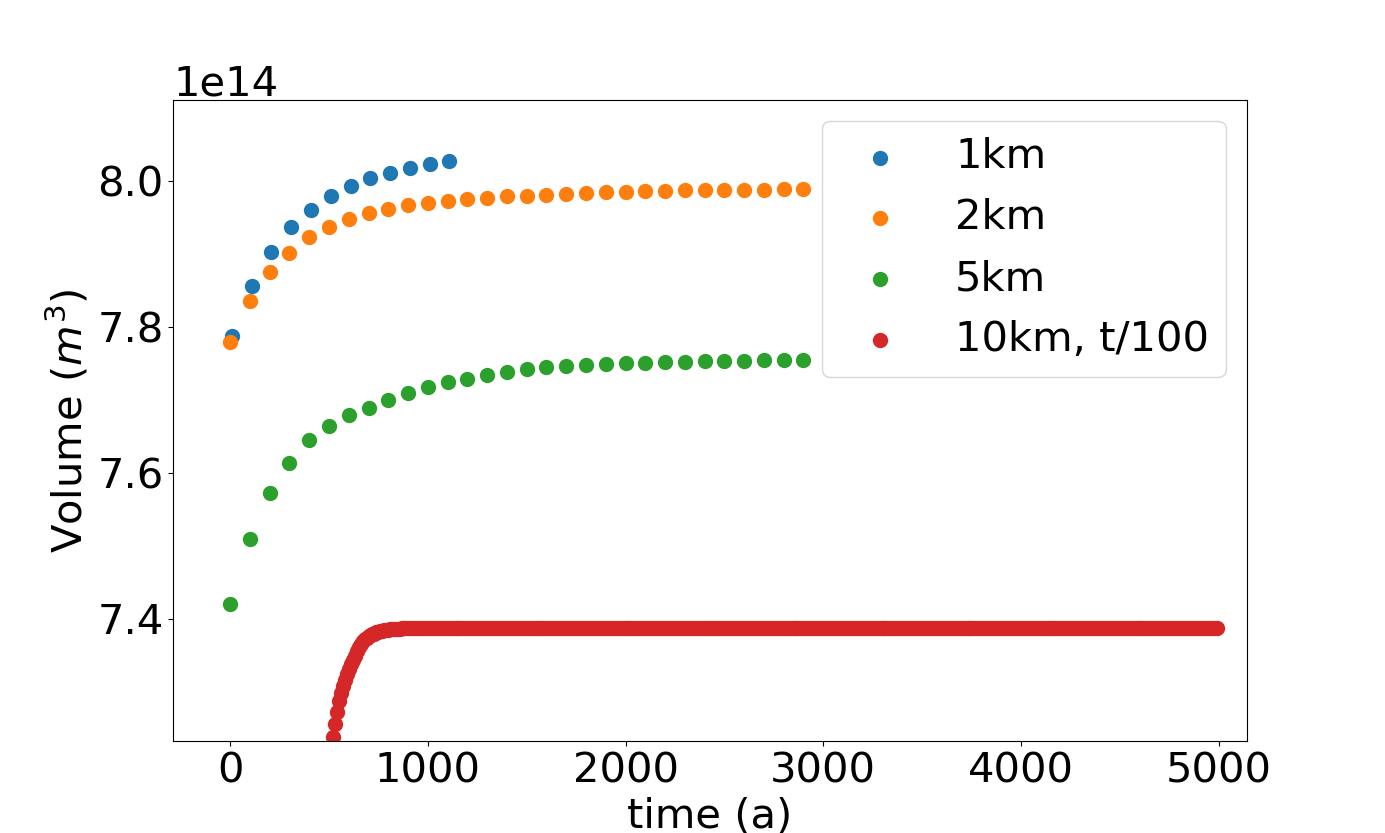
\includegraphics[width=1.1\linewidth]{../fig/Volume_CONE_full_all_res_vs_time.png}
		\caption{Volume variation in time.}
		\label{VOLUME_CONE_VS_TIME}
	\end{subfigure}%
	\begin{subfigure}{.5\textwidth}
	\centering
	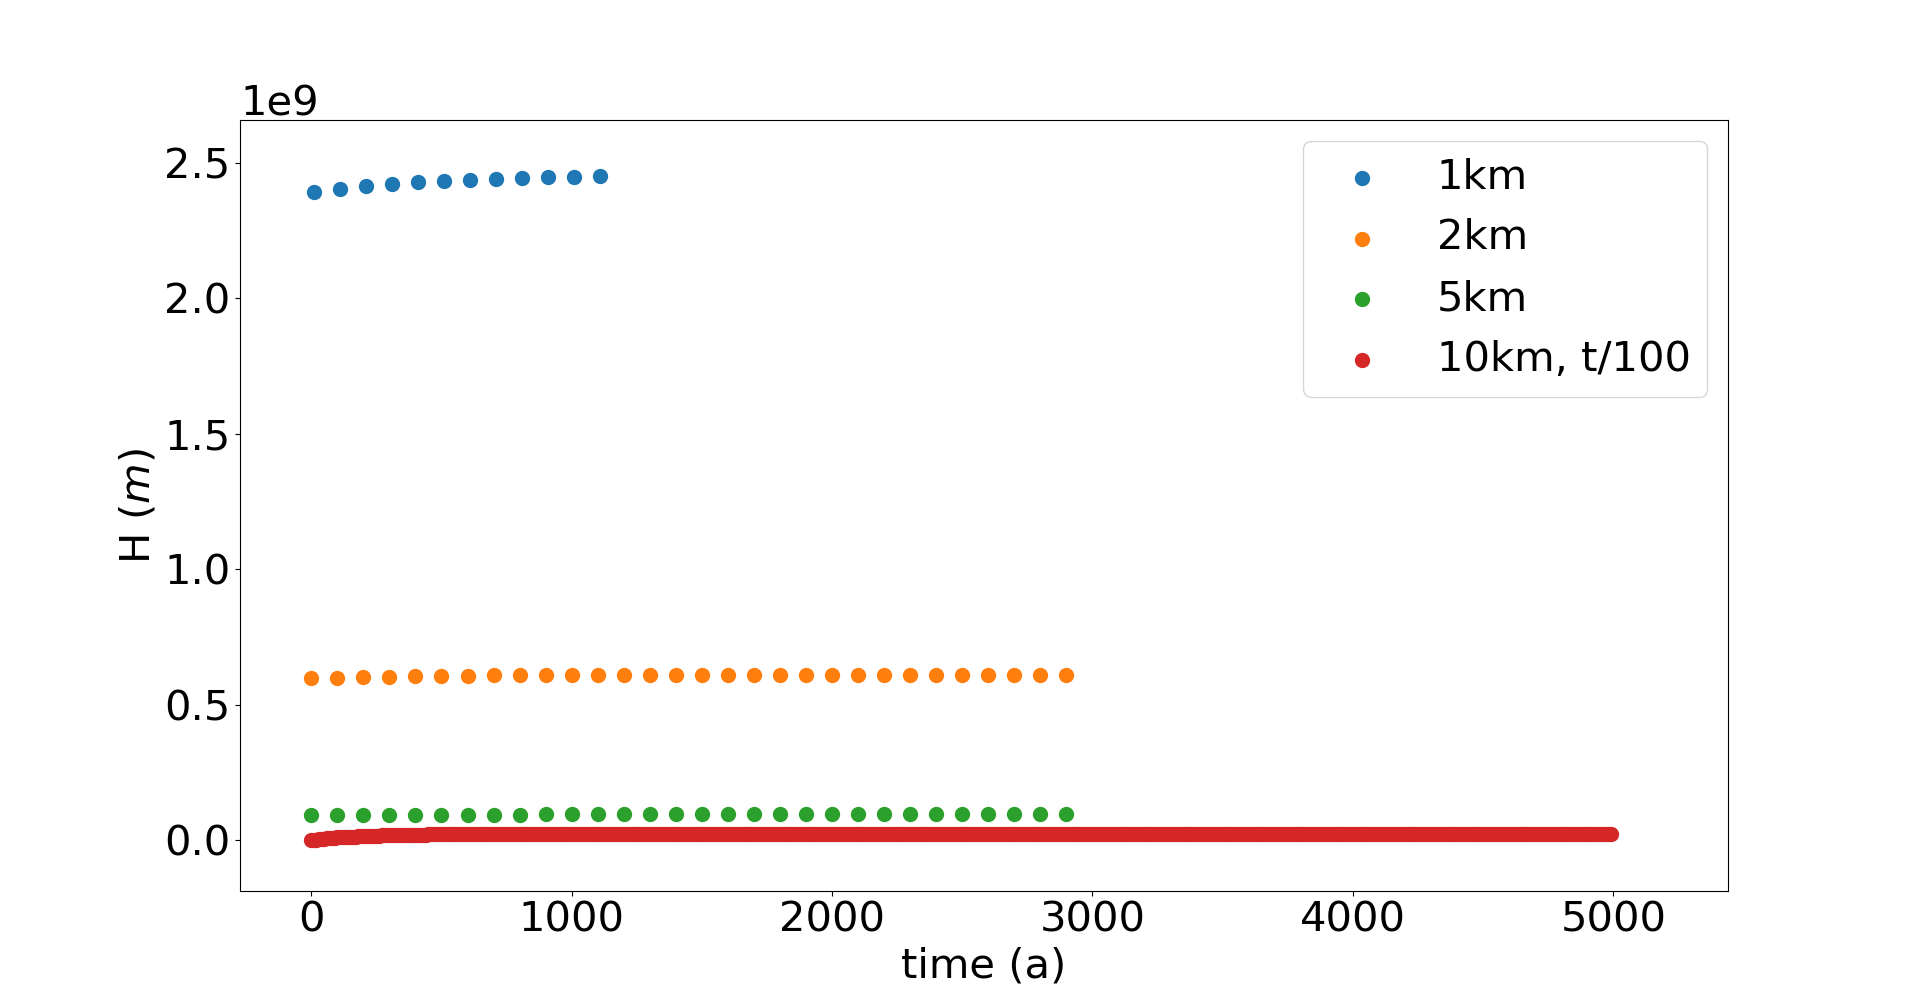
\includegraphics[width=1.1\linewidth]{../fig/H_CONE_full_all_res_vs_time.png}
	\caption{Ice thickess variation in time.}
	\label{H_CONE_VS_TIME}
	\end{subfigure}%
	\caption{Volume variation in time for the cone domain experiment.}
	\label{Volume_CONE_VS_TIME_VS_NODES}
\end{figure}

A different behaviour is observed in figure \ref{H_CONE_VS_NODES} where the ice thickness difference increases as the number of nodes increases, taken as a reference the 1km resolution ice thickness value. This is expected since the ice thickness increases as the resolution does, as observed in figure \ref{H_CONE_VS_TIME}. 

\begin{figure}[!h]
	\centering
	\begin{subfigure}{.45\textwidth}
		\centering
		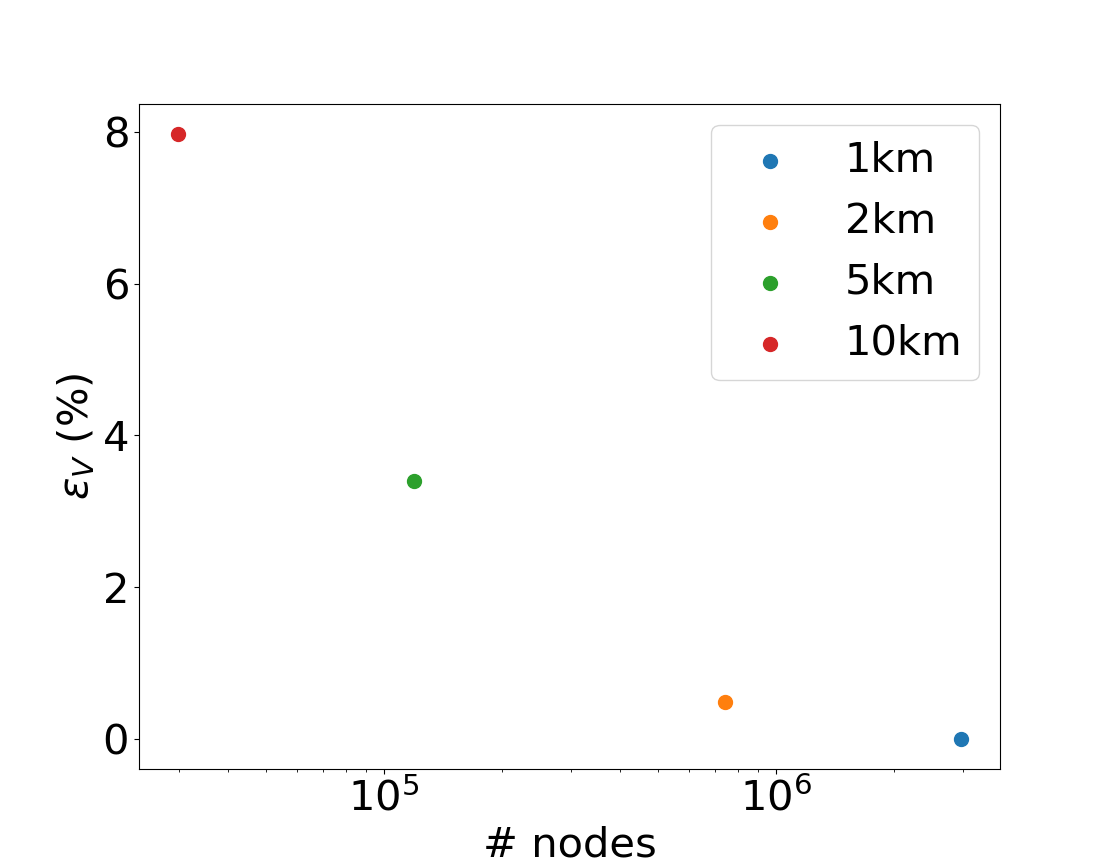
\includegraphics[width=1.1\linewidth]{../fig/Volume_CONE_full_all_res_vs_num_nodes.png}
		\caption{Volume relative variation as a function of the number of nodes.}
		\label{VOLUME_CONE_VS_NODES}
	\end{subfigure}
	\begin{subfigure}{.45\textwidth}
		\centering
		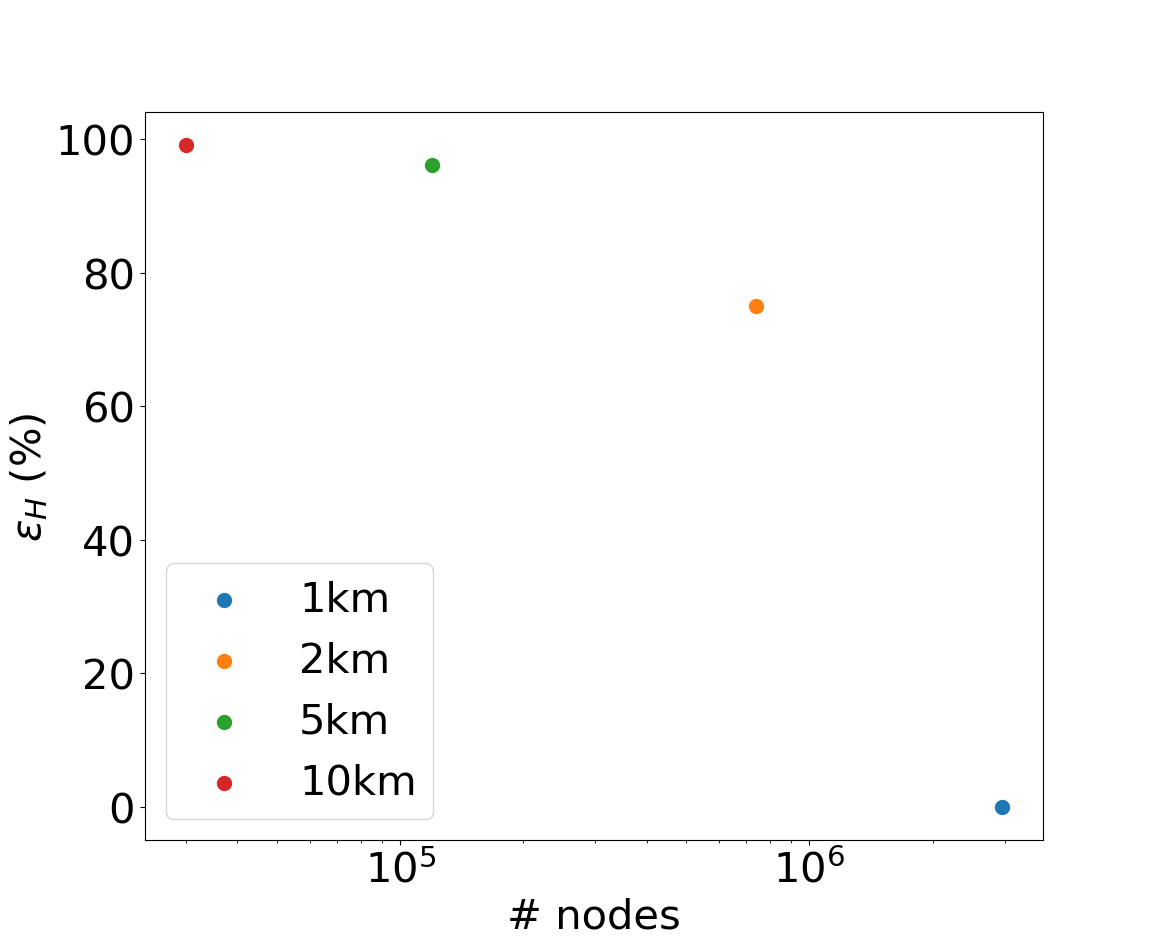
\includegraphics[width=1.1\linewidth]{../fig/H_CONE_full_all_res_vs_num_nodes.png}
		\caption{Ice thickness error as a function of the number of nodes.}
		\label{H_CONE_VS_NODES}
	\end{subfigure}
	\caption{Ice thickess variation in time for the Cone circular domain experiment.}
	\label{H_CONE_VS_TIME_VS_NODES}
\end{figure}

On the other hand, the fact that in figure \ref{VOLUME_CONE_VS_TIME} for each resolution the ice volume starts from the previous resolution volume value, is explained since, to save computational time, each simulation was driven using the previous results as a restart point, so the number of iterations that the solver had to do to reach a steady state was lower for the new resolution. Figure \ref{Computation time} shows the simulation time spent as a function of the number of nodes, where in figure \ref{32_proce} it is shown the simulation time spent using all the 32 processors, while the figure \ref{1_proce} shows the time that would have been spent using only 1 processor, for both experiments cone and thule. The computation time is plotted for 50000 years of simulation. This severally constrained the investigation of the models behaviour with higher resolutions beyond 1 km, since the computation time is plotted in logarithm scale, the time expected for 50000 years of simulation with higher resolution would be a main limitation. For example, it can be observed that to complete a simulation for 1km resolution mesh the computation time would be around 2222 hours with the maximum computational time allowed in the laboratory using the 32 processors, as shown in figure \ref{32_proce}. This time would be 32 times greater if only 1 processor were used (figure \ref{1_proce}).

\begin{figure}[!h]
	\centering
	\begin{subfigure}{.5\textwidth}
		\centering
		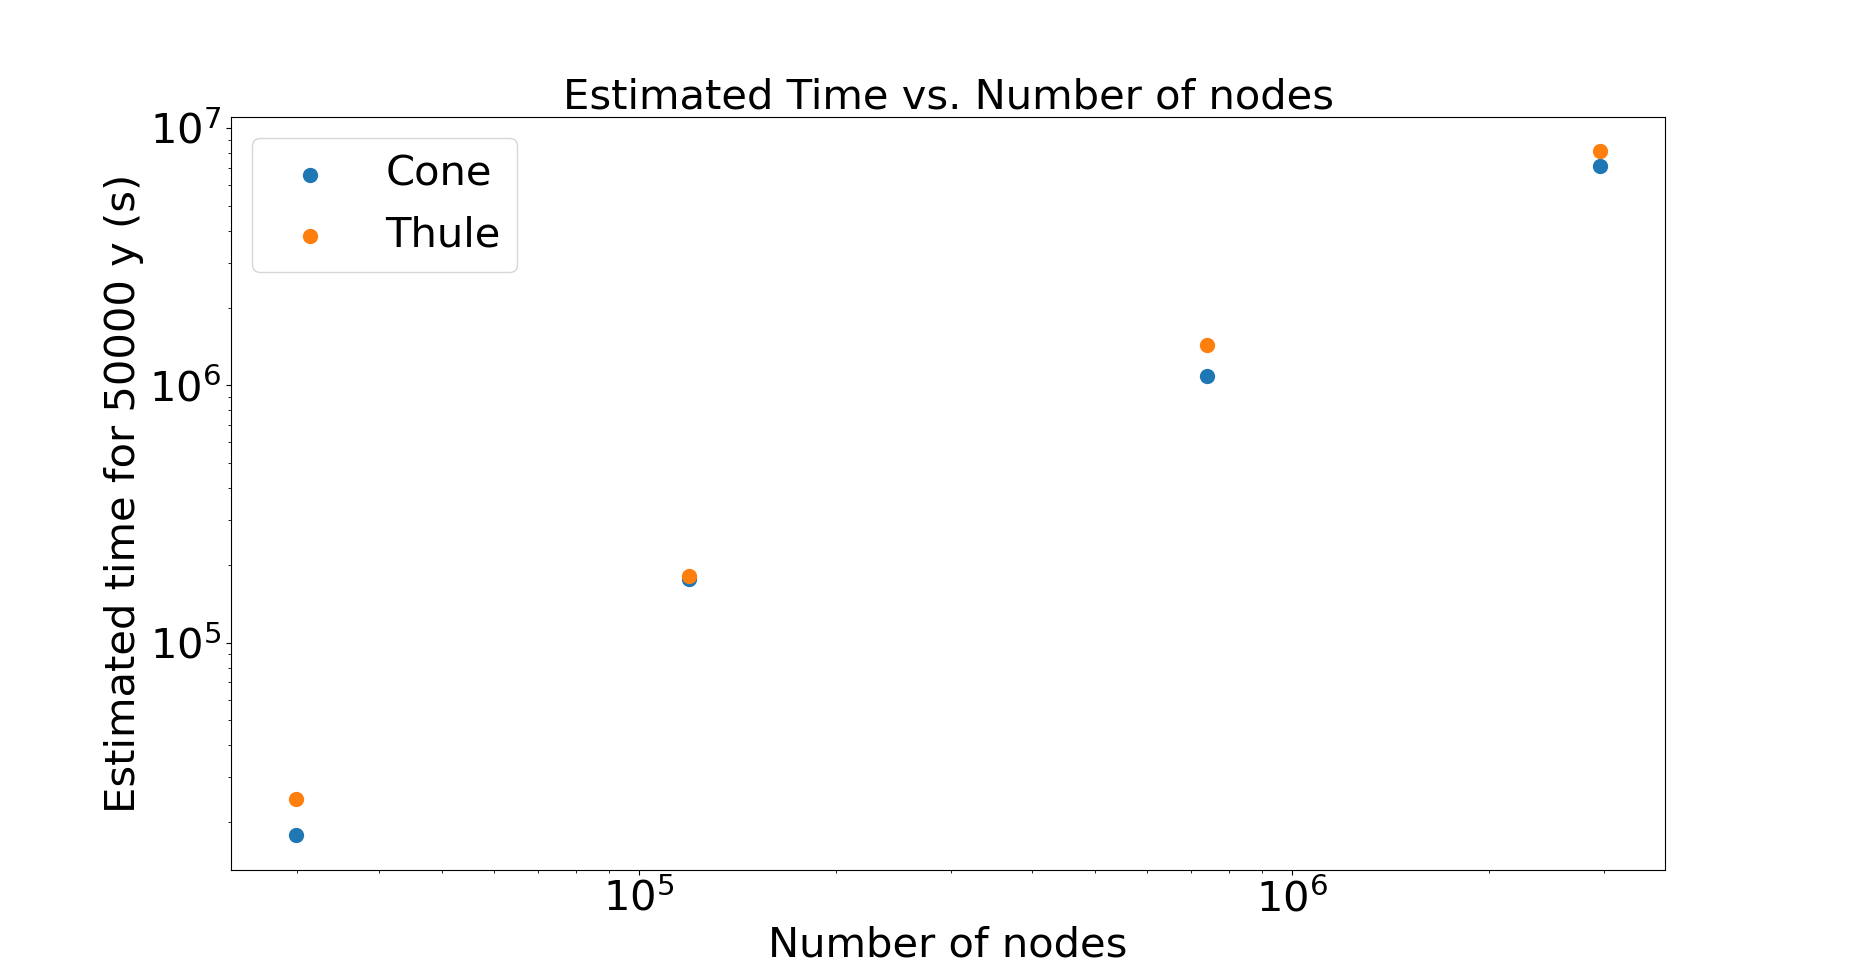
\includegraphics[width=1.1\linewidth]{../fig/Figure_Time_vs_nodes_Segundos.png}
		\caption{Time for 32 processors used.}
		\label{32_proce}
	\end{subfigure}%
	\begin{subfigure}{.5\textwidth}
		\centering
		\includegraphics[width=1.1\linewidth]{../fig/Figure_Time_vs_nodes_32.png}
		\caption{Time for 1 processor.}
		\label{1_proce}
	\end{subfigure}
	\caption{Simulation time as a function of the number of nodes for each resolution mesh.}
	\label{Computation time}
\end{figure}


Figure \ref{figCONO1} shows an schematic representation of the steady state grounded area for the cone experiment, for each resolution. 50km and 20km resolutions simulations are also shown. It can be observed in blue the grounded area and in grey the floating part of the ice. This corresponds to the ice shelf. In this figure it can be directly observed the impact that the resolution mesh has over the prediction of the grounding zone, since starting from the 50km resolution the grounded area has an irregular shape, not axisymmetric and as the resolution increases until 1km resolution, the differences between one resolution and the previous one start to be not that notorious, and also, the grounded area becomes more axisymmetric as expected since the domain is axisymmetric. 

Once the steady state is reached, figure \ref{Grounding_lines__CONE_comparison} shows the position of the grounding line per each resolution, for both the complete and the quarter domain. In this case, per each resolution the mean, maximum and minimum are plotted, as well as the error bar associated for each resolution. The error is set to be half of the resolution. In the y-axis the grounding line position is shown in meters, that is the distance calculated from an origin to the grounding line or grounding zone computed using the grounding line function described previously. This distance is computed as the norm of a vector that defines this grounding line position.  

\begin{figure}[!h]
	\centering % <-- added
	\begin{subfigure}{0.25\textwidth}
		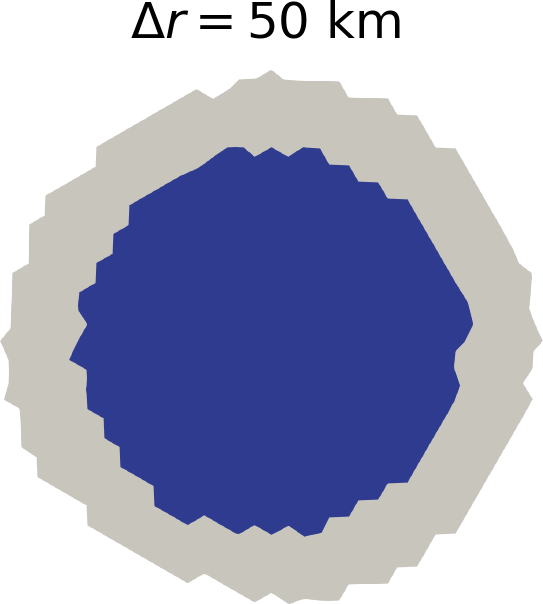
\includegraphics[width=\linewidth]{../fig/Grounded_zone_50km_CONE.png}
		\caption{Grounded zone (blue) and floating ice (grey)}
		\label{figCONE50KM}
	\end{subfigure}\hfil % <-- added
	\begin{subfigure}{0.25\textwidth}
		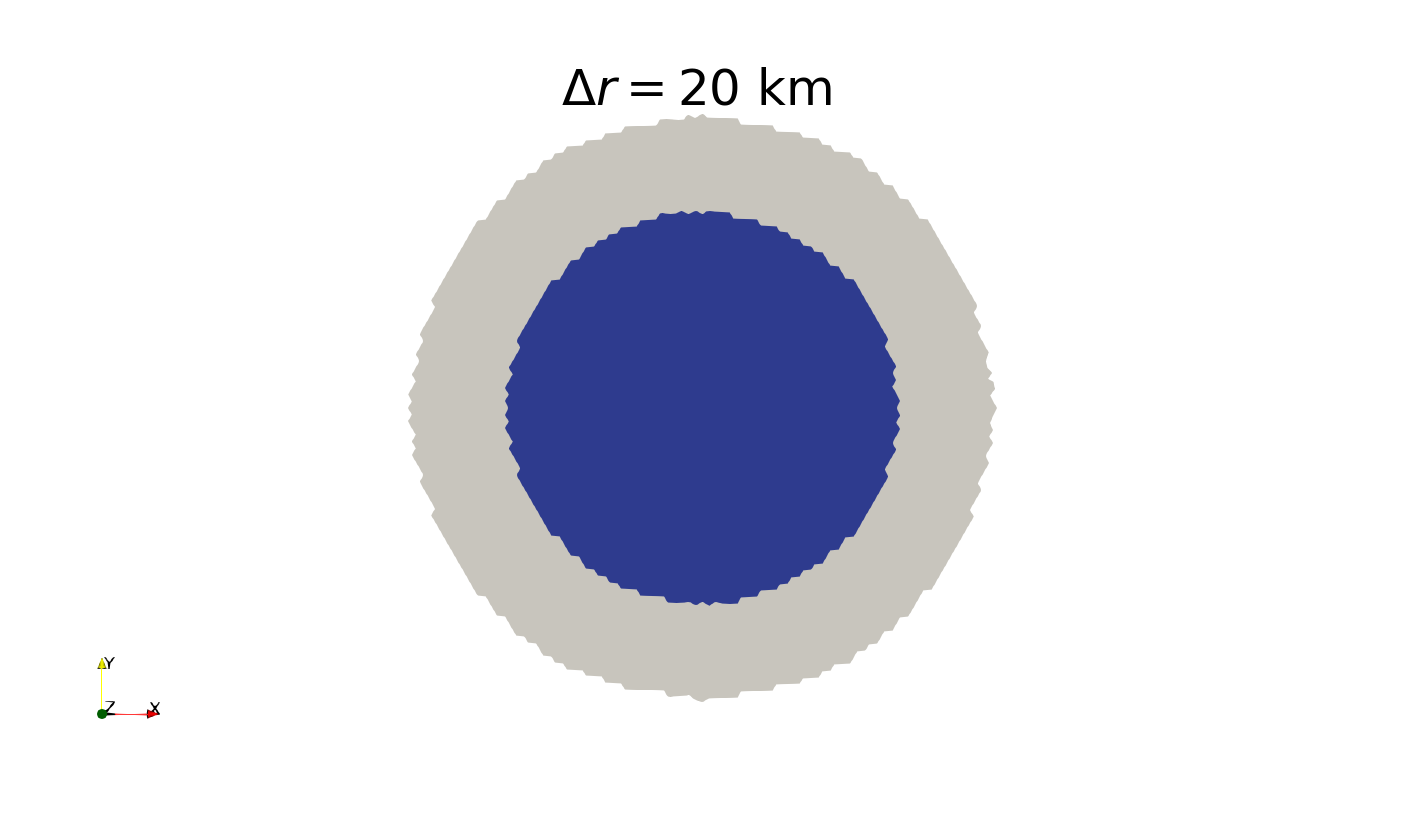
\includegraphics[width=\linewidth]{../fig/Grounded_zone_20km_CONE.png}
		\caption{Grounded zone (blue) and floating ice (grey)}
		\label{figCONE20}
	\end{subfigure}\hfil % <-- added
	\begin{subfigure}{0.25\textwidth}
		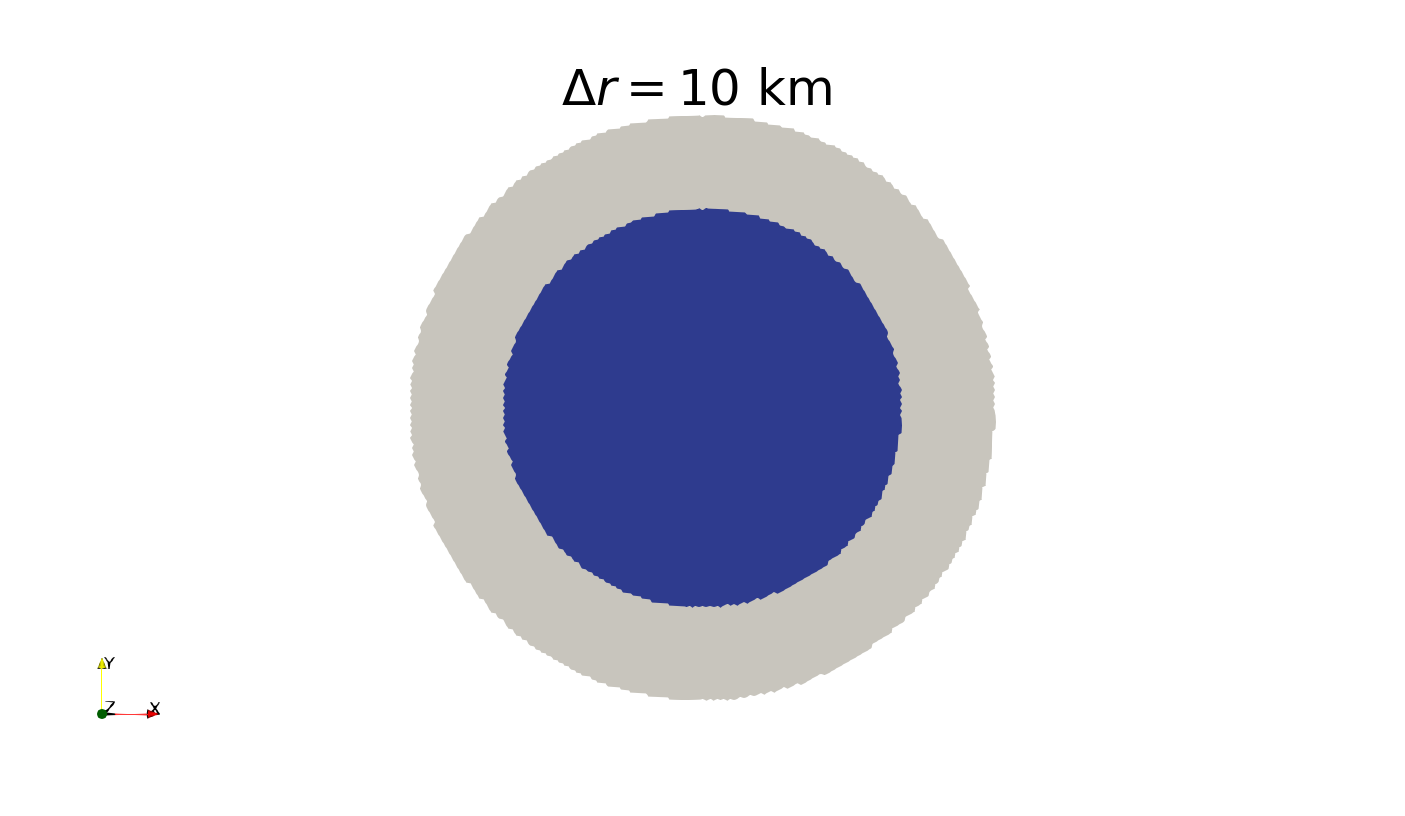
\includegraphics[width=\linewidth]{../fig/Grounded_zone_10km_CONE.png}
		\caption{Grounded zone (blue) and floating ice (grey)}
		\label{figCONE10KM}
	\end{subfigure}
	
	\medskip
	\begin{subfigure}{0.25\textwidth}
		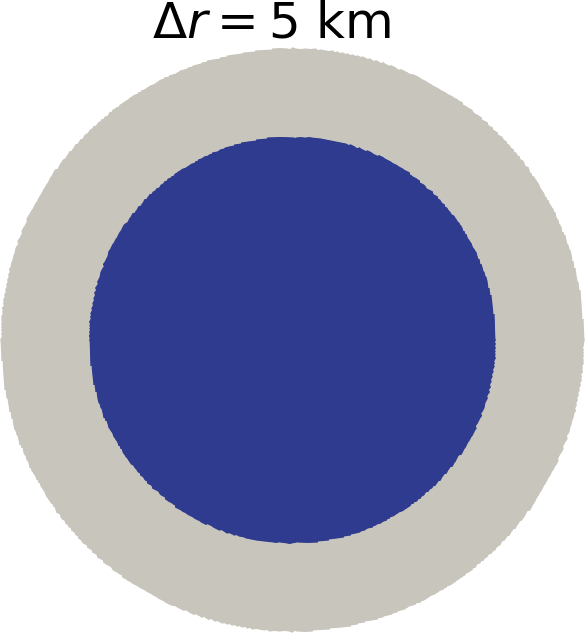
\includegraphics[width=\linewidth]{../fig/Grounded_zone_5km_CONE.png}
		\caption{Grounded zone (blue) and floating ice (grey)}
		\label{figCONE5}
	\end{subfigure}\hfil % <-- added
	\begin{subfigure}{0.25\textwidth}
		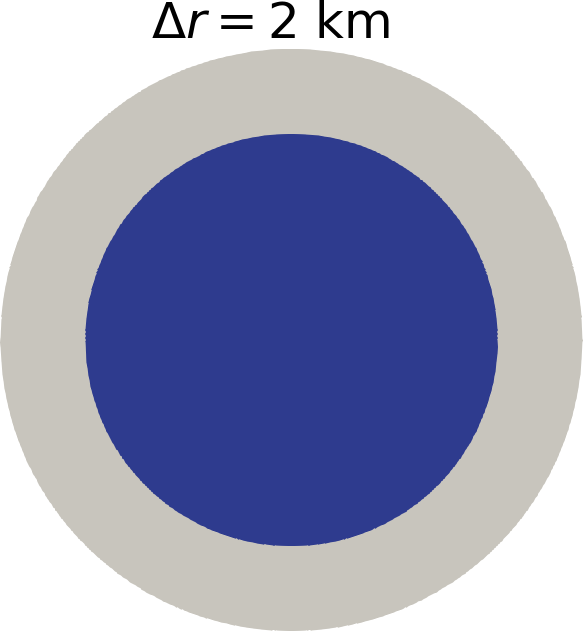
\includegraphics[width=\linewidth]{../fig/Grounded_zone_2km_CONE.png}
		\caption{Grounded zone (blue) and floating ice (grey)}
		\label{figCONE2}
	\end{subfigure}\hfil % <-- added
	\begin{subfigure}{0.25\textwidth}
		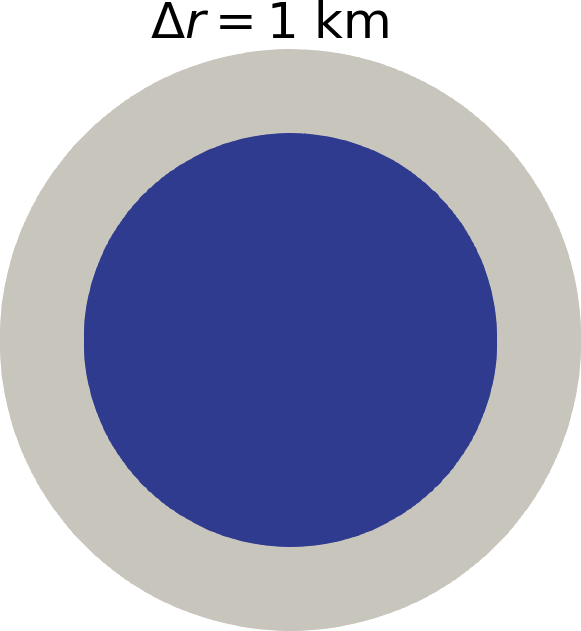
\includegraphics[width=\linewidth]{../fig/Grounded_zone_1km_CONE.png}
		\caption{Grounded zone (blue) and floating ice (grey)}
		\label{CONE1KM}
	\end{subfigure}
	\caption{Grounded zone in blue and floating ice in grey for different resolution mesh in the circular domain.}
	\label{figCONO1}
\end{figure}

\begin{figure}[!h]
	\centering
	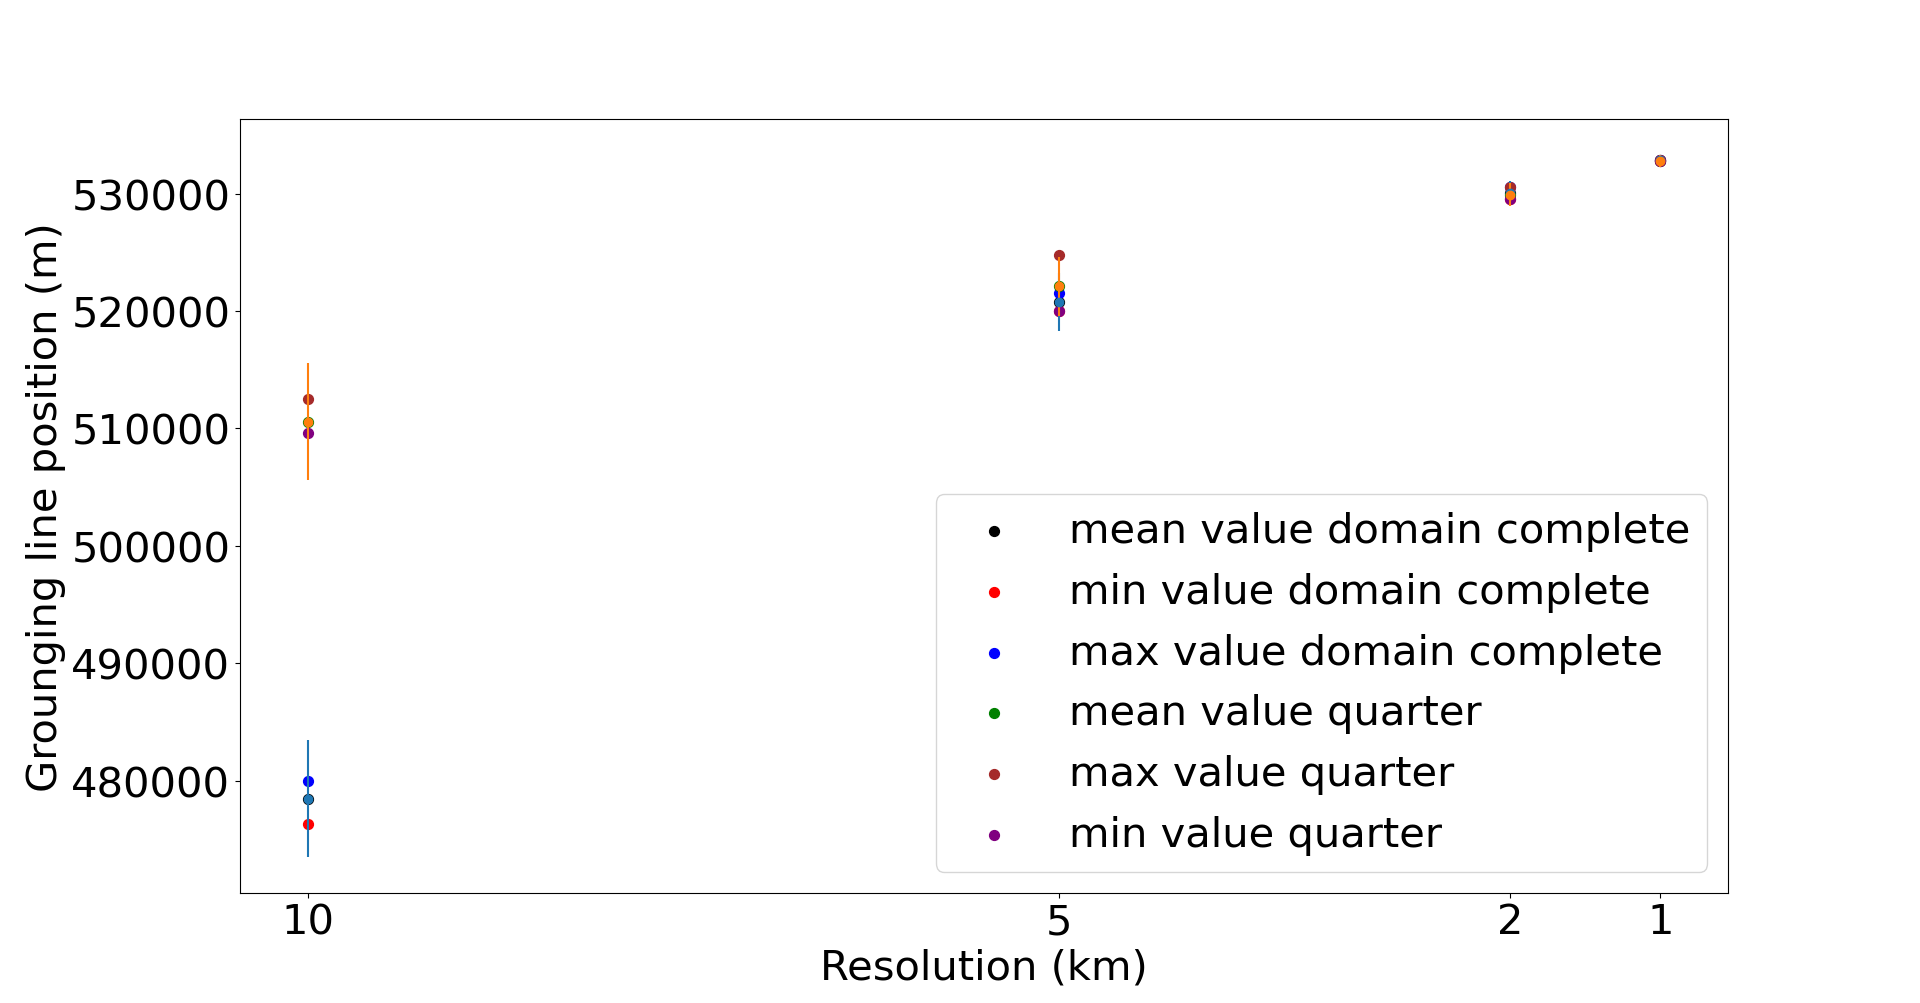
\includegraphics[width=0.8\linewidth]{../fig/Figure_CONE_GL_positions.png}
	\caption{Grounding line positions as a function of the resolution for quarter and complete circular cone domain.}
	\label{Grounding_lines__CONE_comparison}
\end{figure}

There are differences between the grounding line position for the quarter and complete domain for each resolution, and how it starts to decrease as the resolution increases. These results are expected and they match the result shown in figure \ref{figCONO1} where it can be shown that the grounded area is not axisymmetric for very low resolution. Hence, the importance of the comparison between the quarter and complete domain, since it allows to visualize in figure \ref{Grounding_lines__CONE_comparison} the quantitative approach whether the domain is axisymmetric or not. The mean values for the complete domain are computed for all the profiles, while for the quarter domain it is computed for the profiles A, B and C. It can be seen that for higher resolutions (higher than 5km) the differences in the mean values start to decrease. The grounding line position tends to converge to a value as the resolution gets higher. However, further simulations with resolutions higher than 1km should be performed in order to conclude a value for the steady state of the grounding line position, since there are still differences between the grounding line position predicted with the 2km and 1km resolutions, and it is necessary that these differences are 0 or closer to 0 to conclude the independency of the grounding line position to the resolution. 

\begin{figure}[!h]
	\centering
	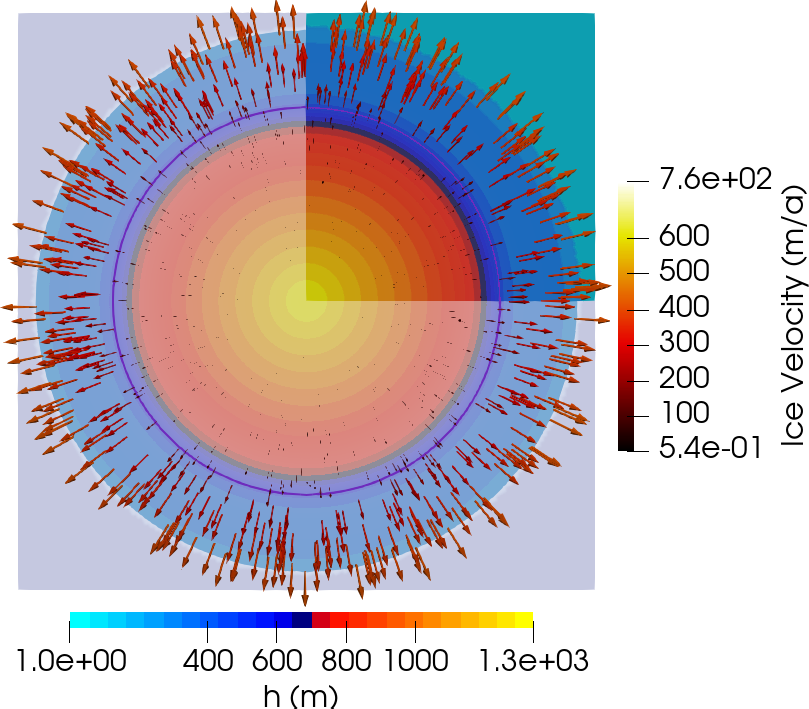
\includegraphics[width=0.6\linewidth]{../fig/Grounding_line_integrated_full_domain-quarter-_CONE_time.png}
	\caption{Ice velocity along the cone spacial domain. The grounded line is highlighted in purple.}
	\label{SSA_velocity}
\end{figure}

In figure \ref{SSA_velocity} the ice velocity in the cone domain experiment is shown, where it can be observed the ice velocity vectors and the magnitude of these as a function of the spacial domain. The quarter of the domain is highlighted and also the grounded zone is highlighted in purple. These velocity vectors are the resultant velocity vectors that come from the computation of the two velocity components using the SSA approximation, and it can be observed that the velocity vectors are radial and perpendicular to the grounding surface highlated in purple. It can be also observed that the velocity has low values in the grounded zone, and then the velocity starts to increase in the ice shelf zones until it reaches the maximum values perpendicularly at the front. This result is expected and corresponds to the fact that the shallow shelf approximation considers the basal shear stress as 0 in the ice shelf that is no longer in contact with the bedrock, so the longitudinal stress dominates, as shown by \cite{allison2009ice}.

In addition to the steady state ice thickness, figure \ref{h_and_h_velocities_cone} shows the ice thickness and the ice thickness rate of change in the spacial domain for the different resolutions. When the resolution starts to be higher, the ice thickness higher differences start to appear in the vicinity of the grounding line. Also, the ice thickness in the ice shelf part of the domain shows more differences for smaller resolutions (10km) radial light blue lines along the ice shelf indicates higher ice thickness in these parts, in comparison with higher resolution where in the ice shelves' part the ice thickness values start to be more uniform. However, despite the fact that there are zones where there are some variations of the ice thickness in the spacial domain, these differences are in a very small range (the largest from the order of 10$^{-3}$m) so it can be concluded the uniformity of the ice thickness values along the domain.


\begin{figure}[!h]
	\centering % <-- added
	\begin{minipage}[t]{.45\textwidth}
		\begin{subfigure}{\textwidth}
			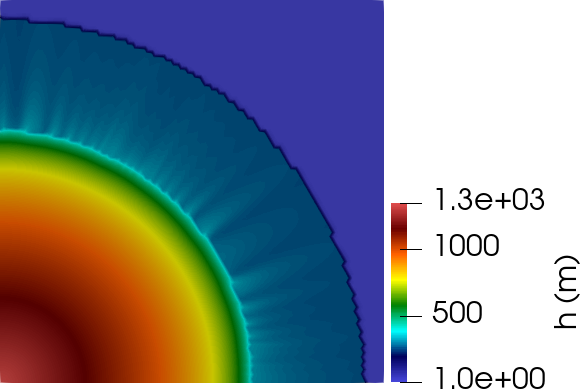
\includegraphics[width=\linewidth]{../fig/10km_quarter_h_thickness_sin_fondo.png}
			\caption{Ice thickness for 10km resolution.}
			\label{h10km}
		\end{subfigure}\hfil % <-- added
		\begin{subfigure}{\textwidth}
			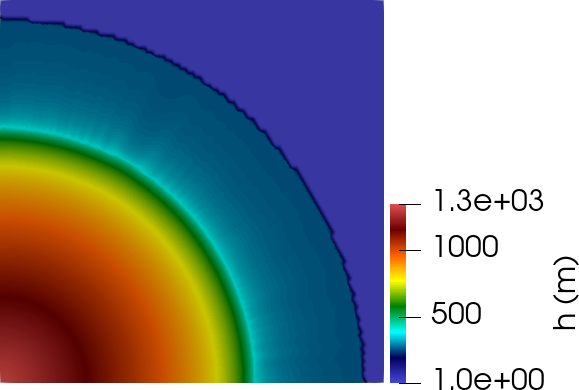
\includegraphics[width=\linewidth]{../fig/5km_quarter_h_thickness_sin_fondo.png}
			\caption{Ice thickness 5km resolution.}
			\label{h5km}
		\end{subfigure}\hfil % <-- added
		\begin{subfigure}{\textwidth}
			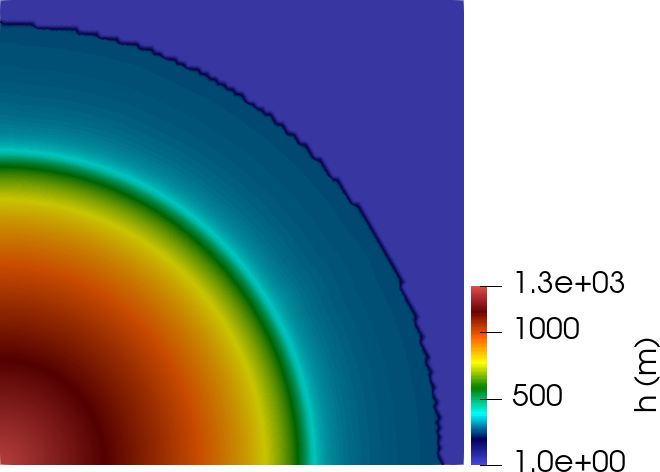
\includegraphics[width=\linewidth]{../fig/2km_quarter_h_thickness_sin_fondo.png}
			\caption{Ice thickness for 2km resolution.}
			\label{h2km}
		\end{subfigure}
		\begin{subfigure}{\textwidth}
		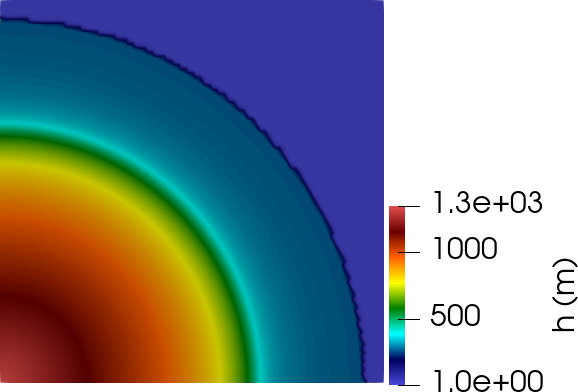
\includegraphics[width=\linewidth]{../fig/1km_quarter_h_thickness_sin_fondo.png}
		\caption{Ice thickness for 1km resolution.}
		\label{h1km}
	    \end{subfigure}
	\end{minipage}\hfil
	\begin{minipage}[t]{.45\textwidth}
		\begin{subfigure}{\textwidth}
			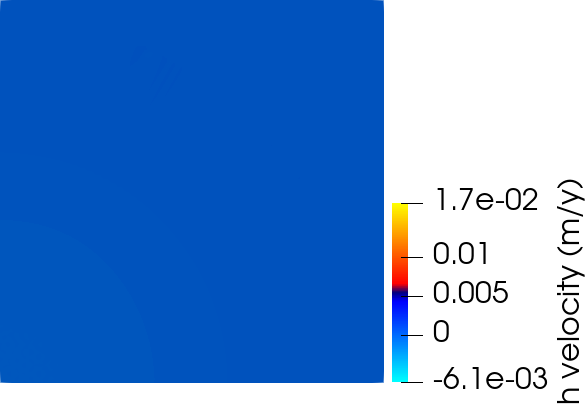
\includegraphics[width=\linewidth]{../fig/10km_quarter_cone_hvelocity_sin_fondo.png}
			\caption{Ice sheet thickness velocity 10km.}
			\label{hvelocity10km}
		\end{subfigure}\hfil % <-- added
		\begin{subfigure}{\textwidth}
			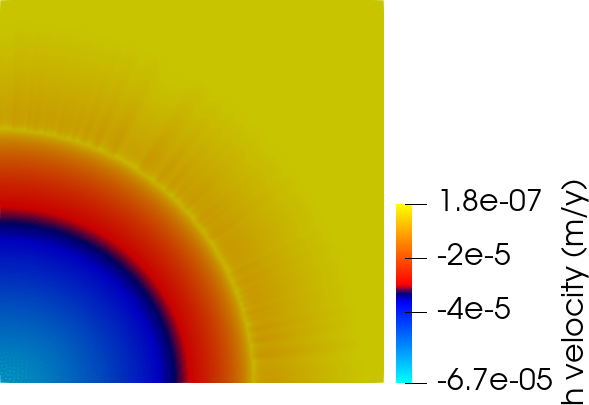
\includegraphics[width=\linewidth]{../fig/5km_quarter_cone_hvelocity_sin_fondo.png}
			\caption{Ice sheet thickness velocity 5km}
			\label{hvelocity5km}
		\end{subfigure}\hfil % <-- added
		\begin{subfigure}{\textwidth}
			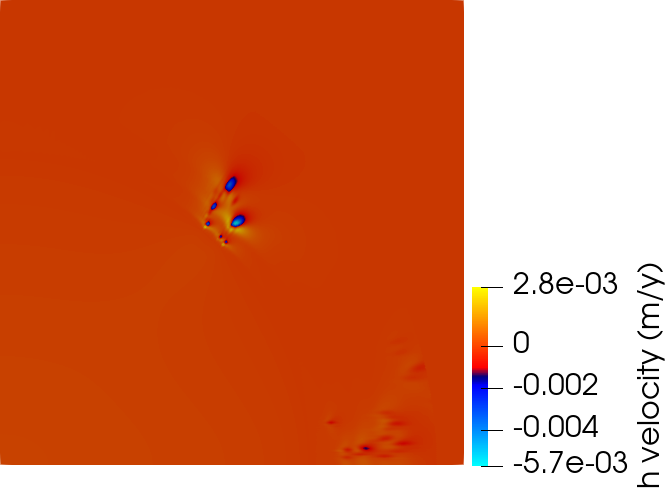
\includegraphics[width=\linewidth]{../fig/2km_quarter_cone_hvelocity_sin_fondo.png}
			\caption{Ice sheet thickness velocity 2km}
			\label{hvelocity2km}
		\end{subfigure}
				\begin{subfigure}{\textwidth}
			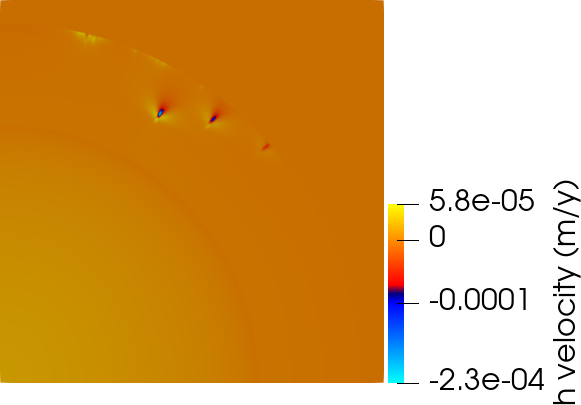
\includegraphics[width=\linewidth]{../fig/1km_quarter_cone_hvelocity_sin_fondo.png}
			\caption{Ice sheet thickness velocity 1km}
			\label{hvelocity1km}
		\end{subfigure}	
	\end{minipage}
	\caption{On the left side, the ice thickness for different resolutions, on the right side; ice sheet thickness rate of change in space for quarter domain per each resolution after steady state.}
	\label{h_and_h_velocities_cone}
\end{figure}

In figure \ref{h_and_h_velocities_cone} the blue dark radial line marks the calving front, so the lighter blue part that its outside of the circumference in this case is not part of the domain.

\subsection{Thule configuration}
For the second part of the experiments, the results for the thule configuration were obtained for a quarter of the domain and the domain complete, and following the CalvingMIP inter-comparison project, the simulations using this topography were run for 10,5,2 and 1 km resolutions. Figure \ref{Thule_profiles_capronas_and_halbranes} shows the schematic representation of the thule domain experiment results. Similar to the Cone domain experiment, in this experiment it is proposed to analyse the results along profiles called Caprona and Halbrane. The figure \ref{Profiles_Thule} highlights the quarter of the domain, since the simulations were also run for this part of the domain to compare it with the complete one, as the domain is symmetric. In this case the results were analysed for Caprona profiles and separately for the Halbrane profiles. In figures \ref{Capronas_thule} and \ref{Halbranes_thule} it can be observed the ice thickness along each one of the profiles and so the position of the grounding line.

\begin{figure}[!h]
  \begin{subfigure}[c]{.52\linewidth}
    \centering
    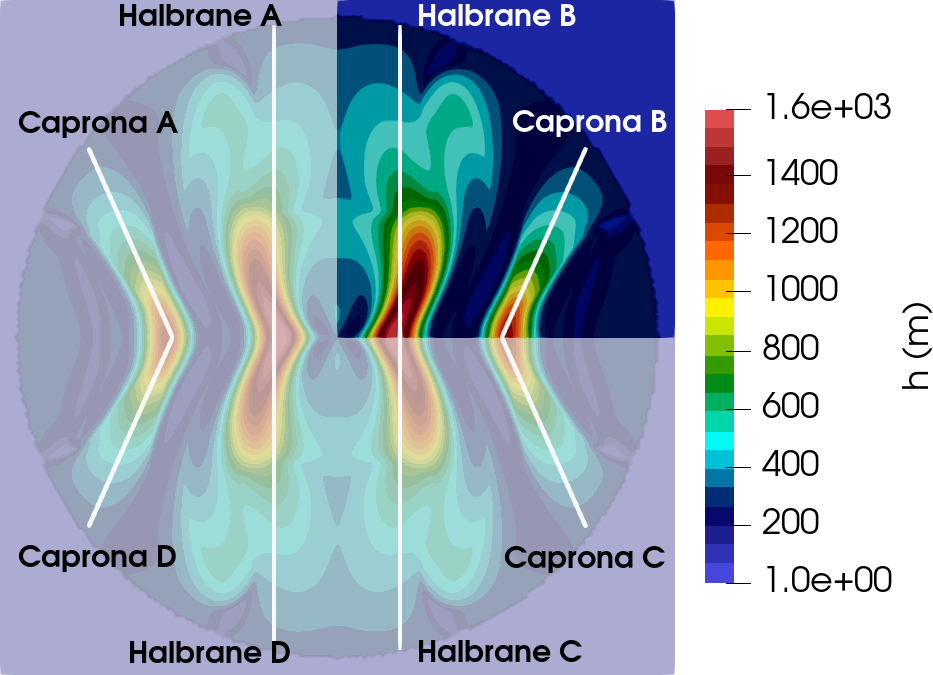
\includegraphics[width=\linewidth]{../fig/Profiles_Thule_combined_domains_2_con_fondo.png}%
    \caption
      {%
        Profiles for the thule domain%
        \label{Profiles_Thule}%
      }%
  \end{subfigure}\hfill
  \begin{tabular}[c]{@{}c@{}}
    \begin{subfigure}[c]{.48\linewidth}
      \centering
      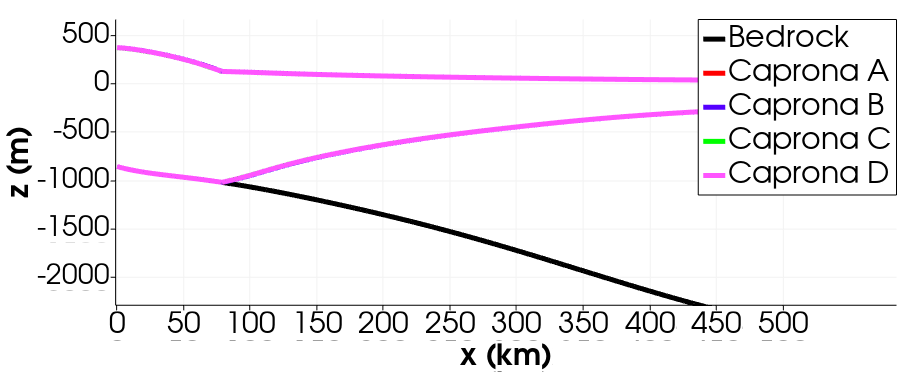
\includegraphics[width=\linewidth]{../fig/Capronas_Thule_Domain_con_fondo.png}%
      \caption
        {%
          Ice thickness along each Caprona profile%
          \label{Capronas_thule}%
        }%
    \end{subfigure}\\
    \noalign{\bigskip}%
    \begin{subfigure}[c]{.48\linewidth}
      \centering
      \includegraphics[width=\linewidth,page=2]{../fig/Halbranes_thule_domain_con_fondo.png}%
      \caption
        {%
          Ice thickness along each Halbrane profile%
          \label{Halbranes_thule}%
        }%
    \end{subfigure}
  \end{tabular}
  \caption
    {%
      Schematic representation of thule ice sheet showing ice thickness along Caprona and Halbrane profiles.%
      \label{Thule_profiles_capronas_and_halbranes}%
    }
\end{figure}

Figure \ref{H_THULE_VS_TIME_VS_NODES} shows the evolution in time of the ice thickness for each one of the resolutions, as well as the ice  volume. It is important to mention that the time domain for the 10km resolution was divided per 10 to make the scale match with the other resolutions results. As the same case for the cone domain experiment, in this case each simulation was driven using the previous resolution result as a restart point, and it can be observed in figure \ref{H_THULE_VS_TIME} that, similarly with the cone domain experiment, the ice thickness increases with the resolution, and for this reason the ice thickness differences are higher once the resolution gets higher (observed in figure \ref{H_THULE_VS_NODES}). 

The different behaviour is observed in figure \ref{VOLUME_THULE_VS_NODES} where the ice volume difference decreases as the number of nodes increases taking as reference the 1km resolution volume, since the figure \ref{VOLUME_THULE_VS_TIME} shows that as the resolution increases, the ice sheet volume tends to converge to a value as it reaches the steady state for each resolution, and the differences between resolutions is every time smaller. 

\begin{figure}[!h]
	\centering
	\begin{subfigure}{.5\textwidth}
		\centering
		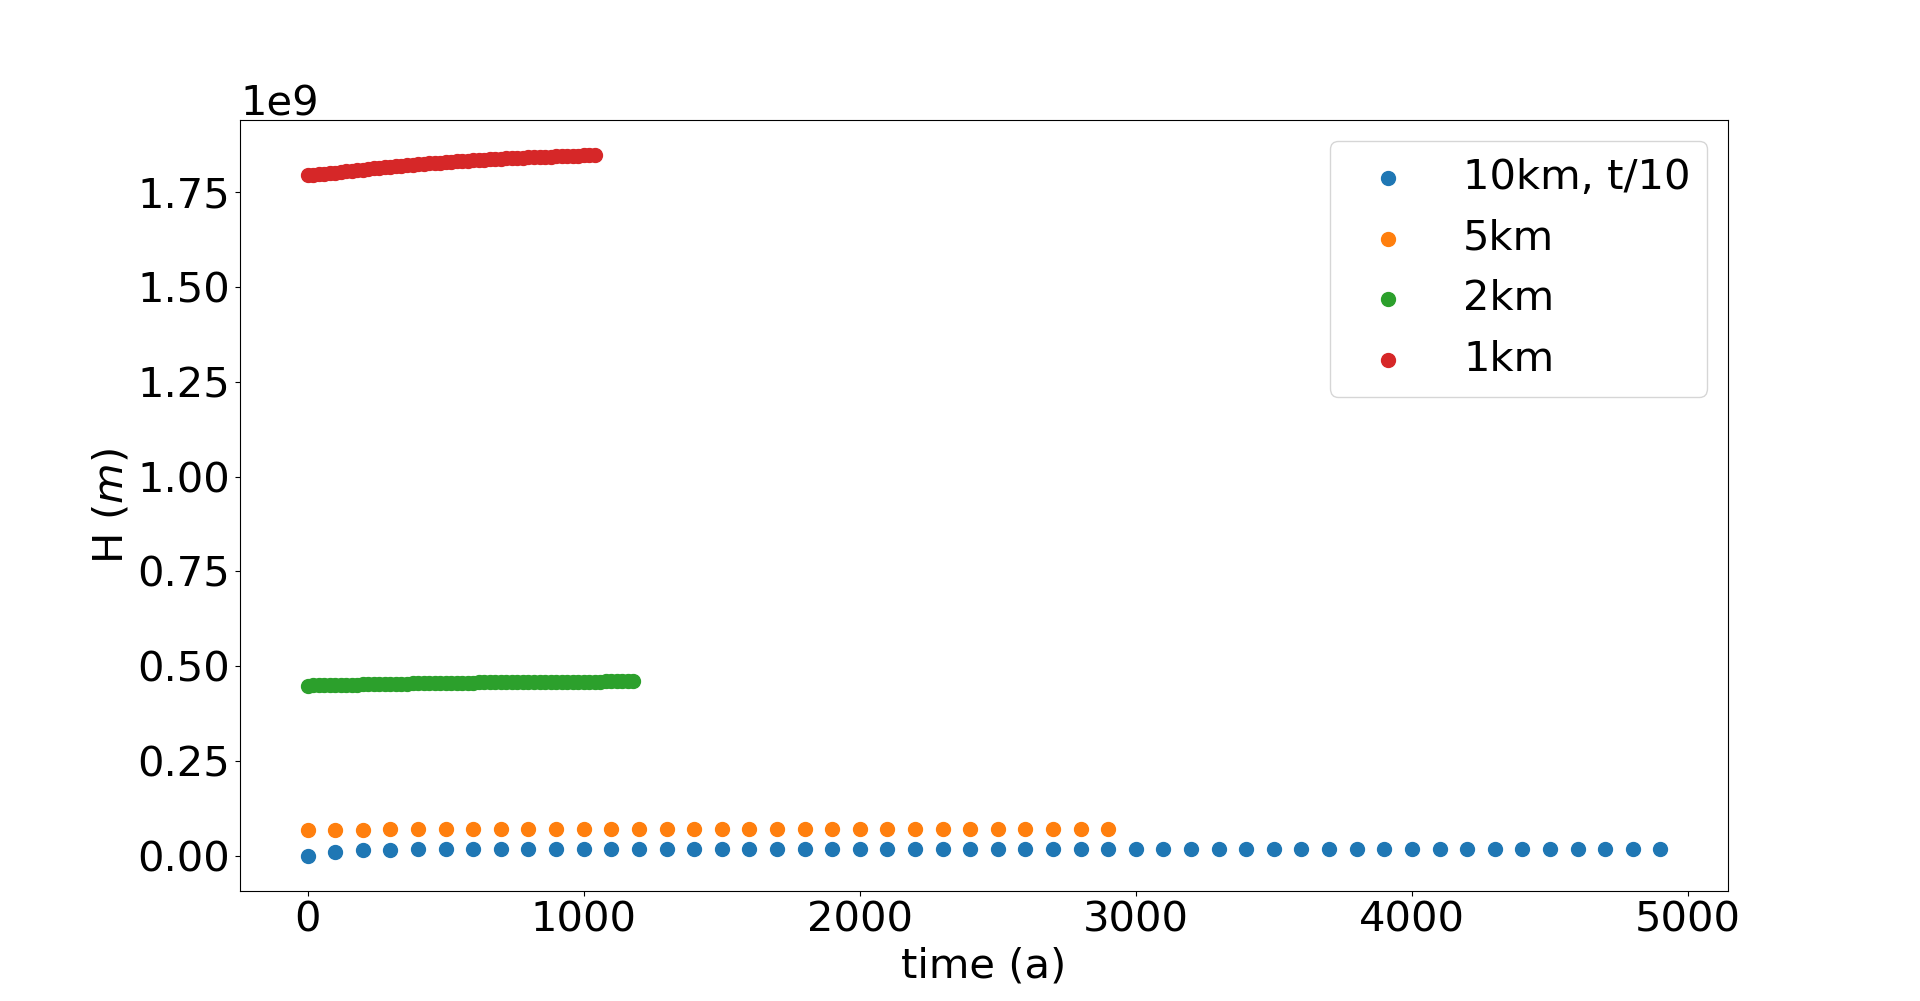
\includegraphics[width=1.1\linewidth]{../fig/H_THULE_full_all_res_vs_time.png}
		\caption{Ice thickess variation in time.}
		\label{H_THULE_VS_TIME}
	\end{subfigure}%
	\begin{subfigure}{.5\textwidth}
	\centering
	\includegraphics[width=1.1\linewidth]{../fig/Volume_THULE_full_all_res_vs_time.png}
	\caption{Volume variation in time.}
	\label{VOLUME_THULE_VS_TIME}
	\end{subfigure}
	\caption{Ice thickess variation in time for the Thule domain experiment.}
	\label{H_THULE_VS_TIME_VS_NODES}
\end{figure}

\begin{figure}[!h]
	\centering
		\begin{subfigure}{.45\textwidth}
		\centering
		\includegraphics[width=1.1\linewidth]{../fig/H_THULE_full_all_res_vs_num_nodes.png}
		\caption{Ice thickness error as a function of the number of nodes.}
		\label{H_THULE_VS_NODES}
	\end{subfigure}
	\begin{subfigure}{.45\textwidth}
		\centering
		\includegraphics[width=1.1\linewidth]{../fig/Volume_THULE_full_all_res_vs_num_nodes.png}
		\caption{Volume relative variation as a function of the number of nodes.}
		\label{VOLUME_THULE_VS_NODES}
	\end{subfigure}
	\caption{Volume variation in time for the thule domain experiment.}
	\label{Volume_THULE_VS_TIME_VS_NODES}
\end{figure}

\begin{figure}[!h]
	\centering % <-- added
	\begin{subfigure}{0.25\textwidth}
		\includegraphics[width=\linewidth]{../fig/Grounded_zone_50km.png}
		\caption{Grounding zone (blue) and floating ice (grey) for 50km resolution.}
		\label{fig:1}
	\end{subfigure}\hfil % <-- added
	\begin{subfigure}{0.25\textwidth}
		\includegraphics[width=\linewidth]{../fig/Grounded_zone_20km.png}
		\caption{Grounding zone (blue) and floating ice (grey) for 20km resolution.}
		\label{fig:2}
	\end{subfigure}\hfil % <-- added
	\begin{subfigure}{0.25\textwidth}
		\includegraphics[width=\linewidth]{../fig/Grounded_zone_10km.png}
		\caption{Grounding zone (blue) and floating ice (grey) for 10km resolution.}
		\label{fig:3}
	\end{subfigure}
	
	\medskip
	\begin{subfigure}{0.25\textwidth}
		\includegraphics[width=\linewidth]{../fig/Grounded_zone_5km.png}
		\caption{Grounding zone (blue) and floating ice (grey) for 5km resolution.}
		\label{fig:4}
	\end{subfigure}\hfil % <-- added
	\begin{subfigure}{0.25\textwidth}
		\includegraphics[width=\linewidth]{../fig/Grounded_zone_2km.png}
		\caption{Grounding zone (blue) and floating ice (grey) for 2km resolution.}
		\label{fig:5}
	\end{subfigure}\hfil % <-- added
	\begin{subfigure}{0.25\textwidth}
		\includegraphics[width=\linewidth]{../fig/Grounded_zone_1km.png}
		\caption{Grounding zone (blue) and floating ice (grey) for 1km resolution.}
		\label{fig:6}
	\end{subfigure}
	\caption{Impact of the resolution in the grounded area.}
	\label{Thule_resolutions}
\end{figure}

For the analysis of these results the same procedure was followed; the simulations were run using a quarter of the domain and the complete one, and the results for the grounding line position were analysed along the profile of Halbrane B and Caprona B for the quarter of the domain. A grounding line function is created and computed as the product of the grounded mask function and the negative of the bedrock position. The negative sign is introduced for the same reason as for the cone domain procedure, since the grounding line is an increasing function and as long as $z_b$ is equal to the bedrock position (namely, the ice sheet is grounded) this product will be negative, so if a negative sign is introduced, it will turn positive, making the inflexion point a unique maximum. This point that represents the position of the grounding line is identified per each resolution and the distance to the origin is calculated, along each one of the profiles Capronas and Halbranes.

The figure \ref{Thule_resolutions} shows a similar scheme of the one done for the circular domain in figure \ref{figCONO1}, where the grounded area and the ice shelf can be observed per each resolution, being the grounded area the blue part. In this case, due to the thule topography, it can be observed that lower resolutions does not even get to identify some zones that actually belong the grounded part (as it can be observed in figure \ref{fig:1} for the 50km resolution mesh, and also for 20 km resolution in figure \ref{fig:2}). Also, due to the topography of the thule, as the resolution increases, actually the grounded area increases, meaning that increasing the resolution grid mesh improves the ability of the model to identify a grounded or not grounded node, that with lower resolutions can be waived. However, for lower resolutions than 5 km it can be observed that the grounded area results start to be consisted and the differences start to decrease.

This fact can be observed when plotting the grounding line position as the function of the resolution along the different profiles. For this experiment, for the quarter of the domain there are only two profiles Caprona B and Halbrane B. For both profiles there is only a value of grounding line position, that is shown in figure \ref{Thule_Capronas} and \ref{Thule_halbranes} respectively. To compare these positions obtained for the quarter domain, the grounding line positions along Halbrane A,B, C and D are computed for the complete domain following the procedure described previously, and the mean, maximum and minimum value per each resolution are listed in figure \ref{Thule_halbranes}. The exact same procedure is applied using the results along the Capronas profiles. For both, the mean value of the grounding line position for the complete domain, and the grounding line position for the quarter domain are shown, the associated error bars are also shown.

\begin{figure}[!h]
	\centering
	\begin{subfigure}{.5\textwidth}
		\centering
		\includegraphics[width=1.1\linewidth]{../fig/Figure_THULE_GLpositions_Capronas.png}
		\caption{Grounding line positions along Capronas profiles.}
		\label{Thule_Capronas}
	\end{subfigure}%
	\begin{subfigure}{.5\textwidth}
		\centering
		\includegraphics[width=1.1\linewidth]{../fig/Figure_THULE_GLpositions_Halbranes.png}
		\caption{Grounding line positions along Halbrane profiles}
		\label{Thule_halbranes}
	\end{subfigure}
	\caption{Grounding line positions as a function of the resolution for quarter and complete thule domain along the Caprona and Halbrane profiles.}
	\label{Grounding_lines__caprona_halbrane_comparison}
\end{figure}

It can be observed that as the mesh resolution increases, the differences between the results for the grounding line positions along both profiles for the complete and quarter domain start to decrease, a similar behaviour observed in the cone circular domain results. However lower differences are observed for the grounding line position along Caprona profiles in comparison with the ones along Halbranes profiles. The grounding line positions along caprona profiles are very similar and results start to be consistent between the full domain and the quarter domain for resolutions higher than 5km. This result matches the one obtained for the cone experiment. This behavior is actually expected, due to the similarity of the topography along caprona profile, and the one along the cone profiles. However, the halbrane profiles are more irregular and the topography along these profiles is not strictly decreasing, as it is the case for the caprona profiles and the cone domain topography. 

\begin{figure}[!h]
	\centering
	\includegraphics[width=0.6\linewidth]{../fig/H_EXP3_colorfull_noProfiles.png}
	\caption{Velocity vectors along the thule spacial domain. The grounded zone is highlighted in purple.}
	\label{SSA_velocity_thule}
\end{figure}

Figure \ref{SSA_velocity_thule} shows the velocity profiles as a function of the spacial domain for the thule experiment. In this case, the velocity vectors obtained are not radial as the ones that were obtained for the first experiment, were it could be observed that the velocity was always perpendicular to the grounded surface. For these experiments, due to the topography of the domain it can be observed how the velocity magnitudes are greater in the center parts of the valleys between the Halbrane A and Halbrane B, for example. Due to the symmetry of the domain, the same case is observed on the opposite part (lower part of the domain). However, it can be observed that the velocity increases in the ice shelf part, once the ice is not grounded, which matches the behavior observed for the cone experiment and it is also expected since in this part the basal shear stress is 0 and the longitudinal stress dominates. 

\section{Discussion and conclusions}

The outcomes of this research have provided insight into the importance of the mesh resolution in the prediction of important parameters like the grounding line position for the glaciers dynamics. The results obtained for the grounding line position for both experiments were consistent with the ones carried out by \cite{durand2009full} were they could show that the grounding line position results start to be consistent for a grid size smaller than 5km. In that case, a Full-Stokes model was implemented, while in this case a Shallow-Shelf approximation was carried out, decreasing the simulation time and the computational resources. For the complete domains, as well as for the quarter domains, the results start to be consistent after 5 km resolution meshes. 

However, this prediction should be interpreted with caution due to the limitations of the current research. As it was mentioned previously, the time spent by the simulations as a function of the number of nodes in the mesh was obtained, showing an exponential behaviour. In these experiments, the results of the simulations were used as a restart for the new resolution simulation, this way the simulations take less time to converge to the final value. For example, for the 2 km resolution simulation for the cone experiment, the difference between the ice thickness in comparison with the 10km resolution ice thickness is around 50\%, meaning that by taking the results of the 10km resolution as a restart point would save this difference in computational time. This is an important remark in order to do further simulations with mesh resolutions higher than 1km.

Besides, even that it has been shown according to the results that a shallow shelf approximation of the Full-Stokes equations can be a good approximation for the prediction of the grounding line position, further experiments with lower mesh resolutions need to be implemented to conclude a robust prediction of these result. 

On the other hand, it could be observed that the steady state ice thickness increases as the resolution mesh increases. This result is expected from the fact that the grounding line position is also increasing as a function of the resolution, as observed in figures \ref{Grounding_lines__CONE_comparison}, \ref{Thule_Capronas} and \ref{Thule_halbranes} for the cone domain, capronas profiles and hablranes profiles for the thule experiment, respectively. Due to the topography of both experiments being in a decreasing slope, it is expected that from very small resolutions to higher ones, the tendency of the model is to find the position of the grounding line in a larger value of $x$, since for the grounding line it must be that $z_b > bedrock$. Once $z_b$ starts being larger than $bedrock$ the ice is set to be not grounded anymore, so this is fixed as the grounding line position. As long as $\Delta x$ or the mesh resolution gets higher, and since the $bedrock$ is a decreasing slope, the new position of the grounding line will be greater than the previous resolution. The fact that the grounding line position increases in a higher resolution, means that the ice thickness will also increase, since the ice column at the grounding line is now larger due to the decreasing slope of the bedrock, meaning that the ice flux through the grounding line will increase. These results matches the theory (\cite{weertman1974stability, schoof2007ice}) that states that the ice flux through the grounding line is dependent on the ice thickness. 

Also, as mentioned before, the groundling line position starts to converge to a value as the resolution gets higher. The results for the grounding line position in figures \ref{Grounding_lines__CONE_comparison} and in figure \ref{Thule_Capronas} can be compared since, as observed, the bedrock topography is similar along the caprona profiles and the cone profiles, however along the halbranes profiles, even if the results start to be very similar between the quarter and the full domain as the resolution increases, there are still some differences as observed in figure \ref{Thule_halbranes}. Further simulations higher than 1km would be needed to conclude the convergence of the grounding line position along the halbranes profiles or to reach a point where the grounding line does not depend on the resolution. This differences are expected since the bedrock topography along these halbranes is not strictly decreasing, so there is more uncertainty to predict the point where $z_b$ becomes larger than the bedrock value. 	Since the differences between the quarter and complete domain grounding line position along halbranes profiles remains around 2km, further resolutions larger than 1km would be needed in order to conclude a grounding line position independent of the mesh resolution along this profile. 

For these reasons, even if the results obtained show that the position of the grounding line can be well predicted using the SSA model for resolution meshes lower than 5km, these results may not indicate enough information about the convergence to a grounding line value independent of the mesh resolution. However, as it was shown, using only a quarter domain can reduce the computation time of further simulations and researches, and these way further simulations beyond 1km resolution meshes can be performed in order to reach to find a stable grounding line position independent of the mesh resolution. In the case of our study, even if the model reached the steady state as shown, for certain topographies there exists still discrepancies between the quarter of the domain and the domain complete for the computation of the grounding line. However, the differences decrease as the mesh resolution increases. It is then encouraging to continue working in the development of models using lower resolutions using previous simulations results as restarting points to try to reach to a resolution where the grounding line position after reaching steady state is the same. This may allow to model systems and domains with even more complicated topographies. 

In this project an approach using a shallow shelf approximation (SSA) model was proposed to simulate the motion of glaciers with two different configuration topography. The ice flow is determined by solving the Stokes problem implemented in finite element code Elmer/Ice with the SSA assumptions. This problem was solved by taking into account the complete domain and also solving only a quarter of the domain, due to the symmetry of the system. The position of the grounding line was studied for different resolution meshes starting from 10km and up to 1km, and it was shown that despite the sensitivity of the grounding line to the mesh resolution, it started to converge for resolutions lower to 5km, despite the configuration or the topography as well. The results for the quarter domain for both topographies showed consistency with the results for the complete domain for the prediction of the grounding line position. However, further simulations need to be performed with resolution meshes lower than 1km to fully conclude the convergence of the grounding line position along all the profiles of the domains. According to the results obtained in this research project, it can be a good path for future researches to run simulation experiments with a quarter of the domain to save computational time, using meshes resolution lower than 5km as the results are consistent due to the symmetry, and it can be possible to model more realistic glacier topographies using SSA models. Developing approaches to model more realistic glacier topographies, can allowed to better understand and predict the dynamics of the glaciers along time, and this way it can be better understood its impact on the formation and changes of the ice sheets and their behaviour. 

\section{Acknowledgments} 

This research is part of the CalvingMIP intercomparison project proposed as part of the  PROTECT (projecting sea-level rise: from ice sheet to local implications), an EU project funded to assess and project changes in the land-based cryosphere, with fully quantified uncertainties to produce robust global, regional and local projections on a range of timescales. All the computations and simulations run and presented in this project were performed in the Institut des géosciences de l'environnement (IGE) and the Observatoire des sciences de l'univers de Grenoble (OSUG-B).

\pagebreak
\bibliographystyle{apalike}
\bibliography{./biblio}
\end{document}


